% Created 2021-10-30 Sat 16:38
\documentclass[9pt, b5paaper]{book}
\usepackage[UTF8]{ctex}
\usepackage{xltxtra}
\usepackage{bera}
\usepackage[T1]{fontenc}
\usepackage[scaled]{beraserif}
\usepackage[scaled]{berasans}
\usepackage[scaled]{beramono}
\usepackage{graphicx}
\usepackage{xcolor}
\usepackage{multirow}
\usepackage{multicol}
\usepackage{float}
\usepackage{textcomp}
\usepackage{geometry}
\geometry{left=1.2cm,right=1.2cm,top=1.5cm,bottom=1.2cm}
\usepackage{algorithm}
\usepackage{algorithmic}
\usepackage{latexsym}
\usepackage{natbib}
\usepackage{minted}
\newminted{common-lisp}{fontsize=ootnotesize}
\usepackage[xetex,colorlinks=true,CJKbookmarks=true,linkcolor=blue,urlcolor=blue,menucolor=blue]{hyperref}
\author{deepwaterooo}
\date{\today}
\title{LeetCode Online Coding Interview Questions -- 错题集}
\hypersetup{
  pdfkeywords={},
  pdfsubject={},
  pdfcreator={Emacs 27.1 (Org mode 8.2.7c)}}
\begin{document}

\maketitle
\tableofcontents


\chapter{sliding window}
\label{sec-1}
\section{1438. Longest Continuous Subarray With Absolute Diff Less Than or Equal to Limit - Medium 双端队列}
\label{sec-1-1}
Given an array of integers nums and an integer limit, return the size of the longest non-empty subarray such that the absolute difference between any two elements of this subarray is less than or equal to limit.

\begin{itemize}
\item 这道题希望有一个用两个双端队列的解法,补出来
\end{itemize}

\begin{minted}[frame=lines,fontsize=\scriptsize,linenos=false]{java}
public class MaxSeg {
    List<Integer> tree = new ArrayList<>();
    int n;
    public MaxSeg (int [] arr) {
        n = arr.length;
        tree = new ArrayList<>(2 * n);
        for (int i = 0; i < n; i++)
            tree.add(0);
        for (int i = 0; i < n; i++)
            tree.add(arr[i]); // same effect as below
        for (int i = n-1; i >= 0; i--) // i >= 0
            tree.set(i, Math.max(tree.get(2 * i), tree.get(2 * i+1)));
    }
    public void update(int idx, int v) {
        idx += n;
        tree.set(idx, v);
        while (idx > 1) {
            idx /= 2;
            tree.set(idx, Math.max(tree.get(2 * idx), tree.get(2 * idx+1)));
        }
    }
    public int getMax(int l, int r) {
        l += n;
        r += n;
        int max = Integer.MIN_VALUE;
        while (l < r) {
            if ((l & 1) == 1) {
                max = Math.max(max, tree.get(l));
                l++;
            }
            if ((r & 1) == 1) {
                r--; // order matters !!!
                max = Math.max(max, tree.get(r));
            }
            l >>= 1;
            r >>= 1;
        }
        return max;
    }
}        
public class MinSeg {
    List<Integer> tree = new ArrayList<>();
    int n;
    public MinSeg (int [] arr) {
        n = arr.length;
        tree = new ArrayList<>(2*n);
        for (int i = 0; i < n; i++) 
            tree.add(0);
        for (int i = 0; i < n; i++) 
            tree.add(arr[i]); 
        for (int i = n-1; i >= 0; i--)  // i >= 0
            tree.set(i,  Math.min(tree.get(2*i),  tree.get(2*i+1)));
    }
    public void update(int idx,  int v) {
        idx += n;
        tree.set(idx,  v);
        while (idx > 1) {
            idx /= 2;
            tree.set(idx,  Math.min(tree.get(2*idx),  tree.get(2*idx+1)));
        }
    }
    public int getMin(int l,  int r) { // [l, r) include left, not included right
        l += n;
        r += n;
        int min = Integer.MAX_VALUE;
        while (l < r) {
            if ((l & 1) == 1) {
                min = Math.min(min,  tree.get(l));
                l++;
            }
            if ((r & 1) == 1) {
                r--; // order matters !!!
                min = Math.min(min,  tree.get(r));
            }
            l >>= 1;
            r >>= 1;
        }
        return min;
    }
}
public int longestSubarray(int[] arr, int limit) { // 单调递增队列,左小右大,右进左出 
    MaxSeg max = new MaxSeg(arr);
    MinSeg min = new MinSeg(arr);
    int res = 0, tmp = 0, j = 0;
    int n = arr.length;
    for (int i = 1; i <= n; i++) {
        if (max.getMax(j, i) - min.getMin(j, i) <= limit) {
            tmp = i-j;
            res = Math.max(res, tmp);
        } else 
            while (max.getMax(j, i) - min.getMin(j, i) > limit && j < i) ++j;
    }
    return res;
}
\end{minted}
\section{862. Shortest Subarray with Sum at Least K - Hard}
\label{sec-1-2}
Given an integer array nums and an integer k, return the length of the shortest non-empty subarray of nums with a sum of at least k. If there is no such subarray, return -1.

A subarray is a contiguous part of an array.
\begin{minted}[frame=lines,fontsize=\scriptsize,linenos=false]{java}
public int shortestSubarray(int[] nums, int k) { 
    int n = nums.length;
    int [] sum = new int[n+1];  
    for (int i = 1; i <= n; i++)  
        sum[i] = nums[i-1] + sum[i-1];
    int res = n + 1;
    ArrayDeque<Integer> q = new ArrayDeque<>(); // decreasing sum [] deque
    for (int i = 0; i <= n; i++) {
        while (!q.isEmpty() && sum[i] - sum[q.peekFirst()] >= k)  // 左出:
            res = Math.min(res, i - q.pollFirst()); // 取值了      // 取解
        while (!q.isEmpty() && sum[q.peekLast()] >= sum[i])       // 右出
            q.pollLast();  
        q.offerLast(i);                                           // 当前元素进队列
    }
    return res <= n ? res : -1;
}
\end{minted}

\section{1425. Constrained Subsequence Sum - Hard}
\label{sec-1-3}
Given an integer array nums and an integer k, return the maximum sum of a non-empty subsequence of that array such that for every two consecutive integers in the subsequence, nums[i] and nums[j], where i < j, the condition j - i <= k is satisfied.

A subsequence of an array is obtained by deleting some number of elements (can be zero) from the array, leaving the remaining elements in their original order.

\section{239. Sliding Window Maximum - Hard}
\label{sec-1-4}
You are given an array of integers nums, there is a sliding window of size k which is moving from the very left of the array to the very right. You can only see the k numbers in the window. Each time the sliding window moves right by one position.

Return the max sliding window.

\begin{minted}[frame=lines,fontsize=\scriptsize,linenos=false]{java}
public int[] maxSlidingWindow(int[] arr, int k) {
    int n = arr.length, startWindowIdx = 0;
    ArrayDeque<Integer> q = new ArrayDeque<>(); // 维持一个递减队列
    int [] ans = new int [n - k + 1];
    for (int i = 0; i < n; i++) {
        startWindowIdx = i-k+1;
        while (!q.isEmpty() && i - q.peekFirst() >= k) q.pollFirst();     // 左出q:maintain k size window, 去头:去掉k windows之外的元素
        while (!q.isEmpty() && arr[q.peekLast()] <= arr[i]) q.pollLast(); // 右出q:去掉递减队列尾部所有不大于当前值的元素,就留一个最大值也行
        q.offerLast(i);  // 进q:进后此时q.size() == k 
        if (startWindowIdx >= 0)
            ans[startWindowIdx] = arr[q.peekFirst()]; // 使用递减队列左端最大值
    }
    return ans;
}
\end{minted}
\begin{itemize}
\item 线段树的做法
\end{itemize}
\begin{minted}[frame=lines,fontsize=\scriptsize,linenos=false]{java}
// https://blog.csdn.net/Yaokai_AssultMaster/article/details/79599809
public class MaxSeg {
    List<Integer> tree = new ArrayList<>();
    int n;
    public MaxSeg (int [] arr) {
        n = arr.length;
        tree = new ArrayList<>(2*n);
        for (int i = 0; i < n; i++) 
            tree.add(0);
        for (int i = 0; i < n; i++) 
            tree.add(arr[i]); // same effect as below
        for (int i = n-1; i >= 0; i--) // i >= 0
            tree.set(i, Math.max(tree.get(2*i), tree.get(2*i+1)));
    }
    public void update(int idx, int v) {
        idx += n;
        tree.set(idx, v);
        while (idx > 1) {
            idx /= 2;
            tree.set(idx, Math.max(tree.get(2*idx), tree.get(2*idx+1)));
        }
    }
    public int getMax(int l, int r) {
        l += n;
        r += n;
        int max = Integer.MIN_VALUE;
        while (l < r) {
            if ((l & 1) == 1) {
                max = Math.max(max, tree.get(l));
                l++;
            }
            if ((r & 1) == 1) {
                r--;            // order matters !!!
                max = Math.max(max, tree.get(r));
            }
            l >>= 1;
            r >>= 1;
        }
        return max;
    }
}
public int[] maxSlidingWindow(int[] arr, int k) {
    int n = arr.length;
    MaxSeg mat = new MaxSeg(arr);
    if (n == k) return new int [] {mat.getMax(0, n)};
    int [] res = new int [n-k+1];
    for (int i = 0; i+k <= n; i++) 
        res[i] = mat.getMax(i, i+k);
    return res;
}
\end{minted}

\section{76. Minimum Window Substring}
\label{sec-1-5}
Given two strings s and t of lengths m and n respectively, return the minimum window substring of s such that every character in t (including duplicates) is included in the window. If there is no such substring, return the empty string "".
The testcases will be generated such that the answer is unique.
A substring is a contiguous sequence of characters within the string.
\begin{minted}[frame=lines,fontsize=\scriptsize,linenos=false]{java}
private boolean satisfies(Map<Character, Integer> s, Map<Character, Integer> t) {
    if (s.size() < t.size()) return false;
    for (Map.Entry<Character, Integer> en : t.entrySet()) {
        if (!s.containsKey(en.getKey()) || s.containsKey(en.getKey()) && s.get(en.getKey()) < en.getValue()) return false;
    }
    return true;
}
public String minWindow(String s, String t) {
    int m = s.length();
    int n = t.length();
    if (m < n) return "";
    if (m == 1 && n == 1 && s.charAt(0) != t.charAt(0)) return "";
    if (n == 1) {
        boolean contains = false;
        for (char c : s.toCharArray()) {
            if (c == t.charAt(0)) {
                contains = true;
                break;
            }
        }
        return !contains ? "" : t;
    } 
    Map<Character, Integer> mt = new HashMap<>();
    for (char c : t.toCharArray()) 
        mt.put(c, mt.getOrDefault(c, 0) + 1);
    Map<Character, Integer> ms = new HashMap<>();
    int l = 0, r = 0, i = 0, j = 0, pl = 0;
    String res = "", tmp = "";
    while (i < m) {
        while (i < m && !satisfies(ms, mt)) {
            ms.put(s.charAt(i), ms.getOrDefault(s.charAt(i), 0) + 1);
            ++i;
        }
        if (satisfies(ms, mt)) {
            tmp = s.substring(l, i);
            if (res.equals("") || res.length() > tmp.length()) res = tmp;
        }
        pl = l;
        while (l < i && satisfies(ms, mt)) {
            System.out.println("\nl: " + l);

            ms.put(s.charAt(l), ms.get(s.charAt(l))- 1);
            if (ms.get(s.charAt(l)) == 0) ms.remove(s.charAt(l));
            ++l;
        }
        if (satisfies(ms, mt) || pl != l) {
            tmp = s.substring(l-1, i);
            if (res.equals("") || res.length() > tmp.length()) res = tmp;
        }
        if (i == m) break;
    }
    return res;
}
\end{minted}
\section{632. Smallest Range Covering Elements from K Lists}
\label{sec-1-6}
You have k lists of sorted integers in non-decreasing order. Find the smallest range that includes at least one number from each of the k lists.
We define the range [a, b] is smaller than range [c, d] if b - a < d - c or a < c if b - a == d - c.
\begin{minted}[frame=lines,fontsize=\scriptsize,linenos=false]{java}
// 时间复杂度:O(nk \log k)O(nklogk),其中 nn 是所有列表的平均长度,kk 是列表数量。所有的指针移动的总次数最多是 nknk 次,每次从堆中取出元素和添加元素都需要更新堆,时间复杂度是 O(\log k)O(logk),因此总时间复杂度是 O(nk \log k)O(nklogk)。
// 空间复杂度:O(k)O(k),其中 kk 是列表数量。空间复杂度取决于堆的大小,堆中维护 kk 个元素。
public int[] smallestRange(List<List<Integer>> nums) {
    int n = nums.size();
    int resMin = 0, resMax = Integer.MAX_VALUE;
    int minRg = resMax - resMin;
    int max = Integer.MIN_VALUE;
    int [] next = new int [n]; // 各子链表中比当前idx位数值大的下一个数的下标,即idx+1,初始化全为0
    Queue<Integer> q = new PriorityQueue<>(new Comparator<Integer>() {
            public int compare(Integer idx1, Integer idx2) {
                return nums.get(idx1).get(next[idx1]) - nums.get(idx2).get(next[idx2]);
            }
        });
    for (int i = 0; i < n; i++) {
        q.offer(i); // 0, 1, 2, .... n-1 真神奇呀
        max = Math.max(max, nums.get(i).get(0));
    }
    int minIdx = 0, curRg = 0;
    while (true) {
        minIdx = q.poll(); // 取出的是最小值的子链表的序号,而子链表里的当前最小值所在子链表中的位置存于next[minIdx]中
        curRg = max - nums.get(minIdx).get(next[minIdx]);
        if (curRg < minRg)  {
            minRg = curRg;
            resMin = nums.get(minIdx).get(next[minIdx]);
            resMax = max;
        }
        next[minIdx]++;
        if (next[minIdx] == nums.get(minIdx).size()) break;
        q.offer(minIdx); // 加回去,但是queue里真正比较的值已经变了,变强大了。。。 // 更新最小值的替换值 
        max = Math.max(max, nums.get(minIdx).get(next[minIdx]));  // 更新最大值
    }
    return new int [] {resMin, resMax};
}
// 这里的 BB 序列是什么?我们可以用一个哈希映射来表示 BB 序列—— B[i]
// B[i] 表示 ii 在哪些列表当中出现过,
// 这里哈希映射的键是一个整数,表示列表中的某个数值,
// 哈希映射的值是一个数组,这个数组里的元素代表当前的键出现在哪些列表里。
// 如果列表集合为:
// 0: [-1, 2, 3]
// 1: [1]
// 2: [1, 2]
// 3: [1, 1, 3]
// 那么可以得到这样一个哈希映射
// -1: [0]
// 1: [1, 2, 3, 3]
// 2: [0, 2]
// 3: [0, 3]
public int[] smallestRange(List<List<Integer>> nums) {
    int n = nums.size();
    Map<Integer, List<Integer>> indices = new HashMap<>();
    int xmin = Integer.MAX_VALUE, xmax = Integer.MIN_VALUE;
    for (int i = 0; i < n; i++) {
        for (int v : nums.get(i)) { // 把大链表中出出过的每一个值作键,值为它所存在于的子链表序号链表
            List<Integer> list = indices.getOrDefault(v, new ArrayList<>());
            list.add(i);
            indices.put(v, list);
            xmin = Math.min(xmin, v);
            xmax = Math.max(xmax, v); // 这里得到全局的最小最大值
        }
    }
    int [] freq = new int [n];
    int inside = 0; // cnt # of lists included in miniRanges
    int left = xmin, right = xmin -1;
    int resLeft = xmin, resRight = xmax;
    while (right < xmax) {
        right ++;
        if (indices.containsKey(right)) {
            for (int x : indices.get(right)) {
                freq[x]++;
                if (freq[x] == 1) inside++;
            }
            while (inside == n) { // find ONE satified solution, try to minimize the range
                if (right - left < resRight - resLeft) {
                    resLeft = left;
                    resRight = right;
                }
                if (indices.containsKey(left)) { // sliding the left size towards right
                    for (int v : indices.get(left)) {
                        freq[v]--;
                        if (freq[v] == 0) --inside;
                    }
                }
                left++;
            }
        }
    }
    return new int [] {resLeft, resRight};
}
\end{minted}

\section{480 Sliding Window Median}
\label{sec-1-7}
The median is the middle value in an ordered integer list. If the size of the list is even, there is no middle value. So the median is the mean of the two middle values.
For examples, if arr = [2,3,4], the median is 3.
For examples, if arr = [1,2,3,4], the median is (2 + 3) / 2 = 2.5.
You are given an integer array nums and an integer k. There is a sliding window of size k which is moving from the very left of the array to the very right. You can only see the k numbers in the window. Each time the sliding window moves right by one position.
Return the median array for each window in the original array. Answers within 10-5 of the actual value will be accepted.
\begin{minted}[frame=lines,fontsize=\scriptsize,linenos=false]{java}
public double[] medianSlidingWindow(int[] nums, int k) {
    TreeMap<Integer, Integer> ma = new TreeMap<>();
    TreeMap<Integer, Integer> mb = new TreeMap<>();
    for (int i = 0; i < k; i++) {
        if (i % 2 == 0) {
            mb.put(nums[i], mb.getOrDefault(nums[i], 0) + 1);
            int n = mb.firstKey();
            if (mb.get(n) == 1) mb.remove(n);
            else mb.put(n, mb.get(n) - 1);
            ma.put(n, ma.getOrDefault(n, 0) + 1);
        } else {
            ma.put(nums[i], ma.getOrDefault(nums[i], 0) + 1);
            int n = ma.lastKey();
            if (ma.get(n) == 1) ma.remove(n);
            else ma.put(n, ma.get(n) - 1);
            mb.put(n, mb.getOrDefault(n, 0) + 1);
        }
    }
    double [] res = new double[nums.length-k+1];
    if (k % 2 == 1) res[0] = ma.lastKey();
    else res[0] =  (double)(((long)(ma.lastKey()) + (long)(mb.firstKey())) / 2.0);
    for (int i = 0; i + k < nums.length; i++) {
        ma.put(nums[i+k], ma.getOrDefault(nums[i+k], 0) + 1);
        int n = ma.lastKey();
        if (ma.get(n) == 1) ma.remove(n);
        else ma.put(n, ma.get(n) - 1);
        mb.put(n, mb.getOrDefault(n, 0) + 1);
        if (ma.containsKey(nums[i])) {
            if (ma.get(nums[i]) == 1) ma.remove(nums[i]);
            else ma.put(nums[i], ma.get(nums[i]) - 1);
            int v = mb.firstKey();
            if (mb.get(v) == 1) mb.remove(v);
            else mb.put(v, mb.get(v) - 1);
            ma.put(v, ma.getOrDefault(v, 0) + 1);
        } else {
            if (mb.get(nums[i]) == 1) mb.remove(nums[i]);
            else mb.put(nums[i], mb.get(nums[i]) - 1);
        }
        if (k % 2 == 1) res[i+1] = ma.lastKey();
        else res[i+1] = (double)(((long)(ma.lastKey()) + (long)(mb.firstKey())) / 2.0);
    }
    return res;
}
\end{minted}

\section{826. Most Profit Assigning Work}
\label{sec-1-8}
You have n jobs and m workers. You are given three arrays: difficulty, profit, and worker where:

difficulty[i] and profit[i] are the difficulty and the profit of the ith job, and
worker[j] is the ability of jth worker (i.e., the jth worker can only complete a job with difficulty at most worker[j]).
Every worker can be assigned at most one job, but one job can be completed multiple times.

For example, if three workers attempt the same job that pays \$1, then the total profit will be \$3. If a worker cannot complete any job, their profit is \$0.
Return the maximum profit we can achieve after assigning the workers to the jobs.
\begin{minted}[frame=lines,fontsize=\scriptsize,linenos=false]{java}
// 法一:暴力TreeMap---O(n^2logn)
public int maxProfitAssignment(int[] difficulty, int[] profit, int[] worker) {
    TreeMap<Integer, Integer> m = new TreeMap<>();
    for (int i = 0; i < difficulty.length; i++) 
        m.put(difficulty[i], i);
    int res = 0, idx;
    Integer low;
    for (int i = 0; i < worker.length; i++) {
        low = m.floorKey(worker[i]); // 使用treemap排序的特长
        if (low == null) continue;
        idx = m.get(low);
        for (int j = 0; j < difficulty.length; j++) 
            if (difficulty[j] <= low && profit[j] >= profit[idx])
                idx = j;
        res += profit[idx];
    }
    return res;
}
// 法二:优化的TreeMap---O(nlogn)
// 如果TreeMap里面保存的是每个difficulty[i] 对应的最大的profit,则就可以直接找floorKey对应的value就是对应的要找的value;
// 那么只需要再遍历一次TreeMap,将最大的到目前key位置最大的value放进去就行了
public int maxProfitAssignment(int[] difficulty, int[] profit, int[] worker) {
    TreeMap<Integer, Integer> m = new TreeMap<>();
    for (int i = 0; i < difficulty.length; i++) 
        m.put(difficulty[i], Math.max(m.getOrDefault(difficulty[i], 0), profit[i]));
    int max = 0;
    for (Integer key : m.keySet()) { 
        max = Math.max(max, m.get(key));
        m.put(key, max); //将最大的到目前key位置最大的value放进去
    }
    int res = 0;
    Integer low;
    for (int i = 0; i < worker.length; i++) {
        low = m.floorKey(worker[i]); // 使用treemap排序的特长
        if (low == null) continue;
        res += m.get(low);
    }
    return res;
}
// 法三:Sort + 双指针---O(nlogn)
// 思路就是先将 difficulty[]和profit组成pair,然后再将list和worker[]从小到大排序,然后遍历worker,更新tempMaxProfit,得到总的maxProfit
public int maxProfitAssignment(int[] difficulty, int[] profit, int[] worker) {
    List<int[]> list = new ArrayList<>();
    for (int i = 0; i < difficulty.length; i++) 
        list.add(new int[] {difficulty[i], profit[i]});
    Collections.sort(list, (a, b) -> {return a[0] - b[0];});
    Arrays.sort(worker);
    int res = 0, tmpMaxProfit = 0;
    // i, j同向双指针移动,更新到目前的tmpMaxProfit
    for (int i = 0, j = 0; i < worker.length; i++) {
        while (j < list.size() && list.get(j)[0] <= worker[i]) {
            tmpMaxProfit = Math.max(tmpMaxProfit, list.get(j)[1]);
            j++;
        }
        //此时tmpMaxProfit是前面所有difficulty小于worker[i]的最大的proifit
        res += tmpMaxProfit;
    }
    return res;
}
\end{minted}

\section{1838. Frequency of the Most Frequent Element - Medium}
\label{sec-1-9}
The frequency of an element is the number of times it occurs in an array.

You are given an integer array nums and an integer k. In one operation, you can choose an index of nums and increment the element at that index by 1.

Return the maximum possible frequency of an element after performing at most k operations.

由反证可得,在一定操作次数下最高频元素为原数组中的元素,结合贪心算法,应优先选择不大于该元素的最大数字进行递增操作。

因此,可对原数组排序后,结合双指针算法求解。设计左、右两个指针,在移动右指针的同时,维护左指针的位置,使区间内元素全部递增到右指针所在元素值的操作次数符合要求,此时区间的长度就是该元素的频率。

\begin{minted}[frame=lines,fontsize=\scriptsize,linenos=false]{java}
public int maxFrequency(int[] nums, int k) {
    int n = nums.length, ans = 1, cnt = 0;
    Arrays.sort(nums);
    for (int l = 0, r = 1; r < n; r++) {
        cnt += (nums[r] - nums[r-1]) * (r - l);// 右指针移动后所需操作次数
        while (cnt > k)                        // 操作次数超过k,移动左指针
            cnt -= nums[r] - nums[l++];
        ans = Math.max(ans, r-l+1);            // 区间长度为操作后当前元素的频数
    }
    return ans;
}
\end{minted}

\section{1703. Minimum Adjacent Swaps for K Consecutive Ones - Hard}
\label{sec-1-10}
You are given an integer array, nums, and an integer k. nums comprises of only 0's and 1's. In one move, you can choose two adjacent indices and swap their values.

Return the minimum number of moves required so that nums has k consecutive 1's.

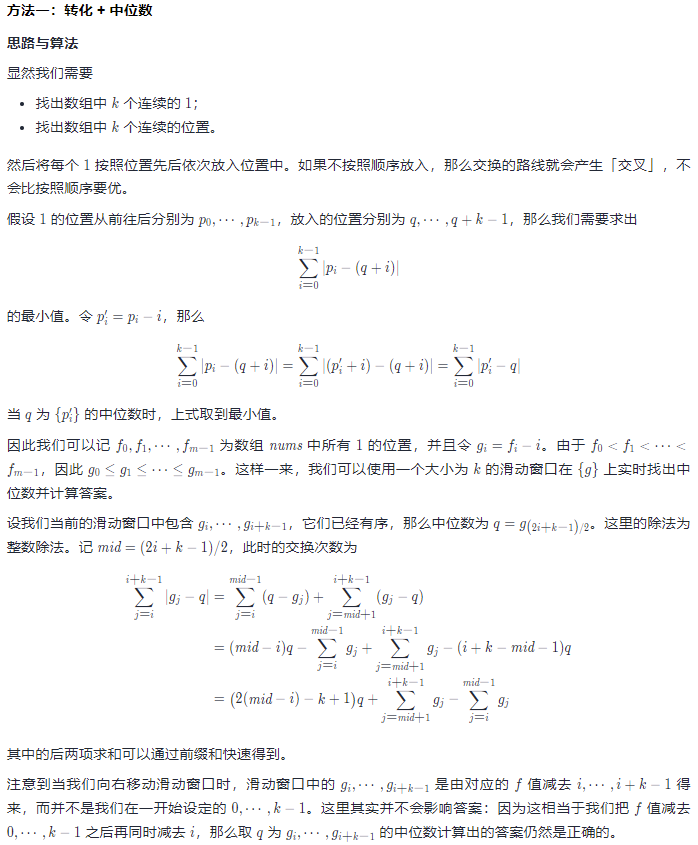
\includegraphics[width=.9\linewidth]{./pic/median.png}

\begin{minted}[frame=lines,fontsize=\scriptsize,linenos=false]{java}
public int minMoves(int[] arr, int k) {
    if (k == 1) return 0;
    int n = arr.length;
    List<Integer> g = new ArrayList<>();
    List<Integer> sum = new ArrayList<>();
    sum.add(0);
    int cnt = -1, last = 0;
    for (int i = 0; i < n; i++) {
        if (arr[i] == 0) continue;
        ++cnt;
        g.add(i-cnt);
        sum.add(last + i - cnt);
        last += i - cnt; 
    }
    int m = g.size();
    int ans = Integer.MAX_VALUE;
    for (int i = 0; i+k <= m; i++) {
        int mid = (i + i + k - 1) / 2; // 中位数下标
        int q = g.get(mid);            // 中位数
        ans = Math.min(ans, (2*(mid-i)-k+1) * q + sum.get(i+k) - sum.get(mid+1) - sum.get(mid) + sum.get(i));
    }
    return ans;
}
\end{minted}
\section{220. Contains Duplicate III - Medium}
\label{sec-1-11}
Given an integer array nums and two integers k and t, return true if there are two distinct indices i and j in the array such that abs(nums[i] - nums[j]) <= t and abs(i - j) <= k.
\begin{minted}[frame=lines,fontsize=\scriptsize,linenos=false]{java}
public boolean containsNearbyAlmostDuplicate(int [] arr, int k, int t) {
    TreeSet<Long> ts = new TreeSet<>();
    for (int i = 0; i < arr.length; i++) {
        if (i >= k+1) ts.remove((long)arr[i-k-1]);
        Long lower = ts.ceiling((long)arr[i]-t); // E ceiling(E e) ,返回 treeSet 中大于等于 e 的元素中最小的元素,如果没有大于等于 e 的元素就返回 null
        if (lower != null && lower <= (long)arr[i] + t)
            return true;
        ts.add((long)arr[i]);
    }
    return false;
}
// 维持一个长度为k的window, 每次检查新的值是否与原来窗口中的所有值的差值有小于等于t的. 如果用两个for循环会超时O(nk).
//     使用treeset( backed by binary search tree) 的subSet函数,可以快速搜索. 复杂度为 O(n logk)
public boolean containsNearbyAlmostDuplicate(int[] nums, int k, int t) {
    if (k < 1 || t < 0 || nums == null || nums.length < 2) return false;
    SortedSet<Long> set = new TreeSet<Long>();
    for(int j = 0; j < nums.length; j++) {
        SortedSet<Long> subSet = set.subSet((long)nums[j] - t, (long)nums[j] + t + 1);
        if (!subSet.isEmpty()) return true;
        if (j >= k)  set.remove((long)nums[j - k]);
        set.add((long)nums[j]);
    }
    return false;
}
\end{minted}


\chapter{backTracking 回溯}
\label{sec-2}
\section{491. Increasing Subsequences}
\label{sec-2-1}
Given an integer array nums, return all the different possible increasing subsequences of the given array with at least two elements. You may return the answer in any order.

The given array may contain duplicates, and two equal integers should also be considered a special case of increasing sequence.
\begin{minted}[frame=lines,fontsize=\scriptsize,linenos=false]{java}
private void dfs(int [] arr, int idx, List<Integer> l) {
    if (l.size() >= 2)
        res.add(new ArrayList<>(l));
    Set<Integer> vis = new HashSet<>();
    for (int i = idx; i < arr.length; i++) {
        if (vis.contains(arr[i])) continue;
        if (l.size() == 0 || arr[i] >= l.get(l.size()-1)) {
            vis.add(arr[i]);
            l.add(arr[i]);
            dfs(arr, i+1, l);
            l.remove(l.size()-1);
        }
    }
}
List<List<Integer>> res = new ArrayList<>();
public List<List<Integer>> findSubsequences(int[] arr) {
    if (arr == null || arr.length == 0) return res;
    dfs(arr, 0, new ArrayList<Integer>());
    return res;
}
\end{minted}


\chapter{排序与recursion}
\label{sec-3}

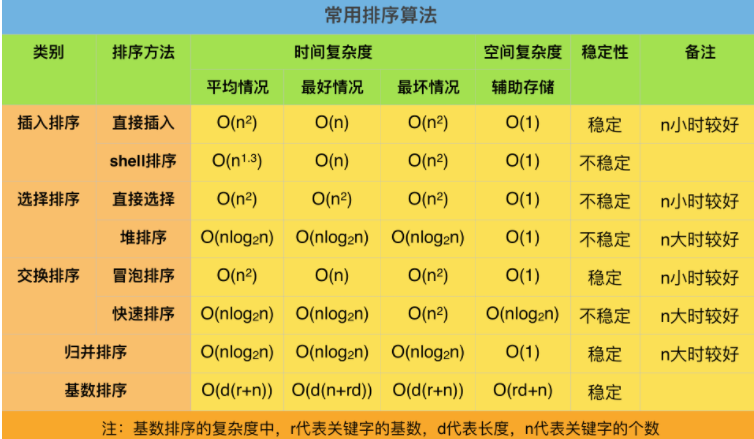
\includegraphics[width=.9\linewidth]{./pic/sort.png}

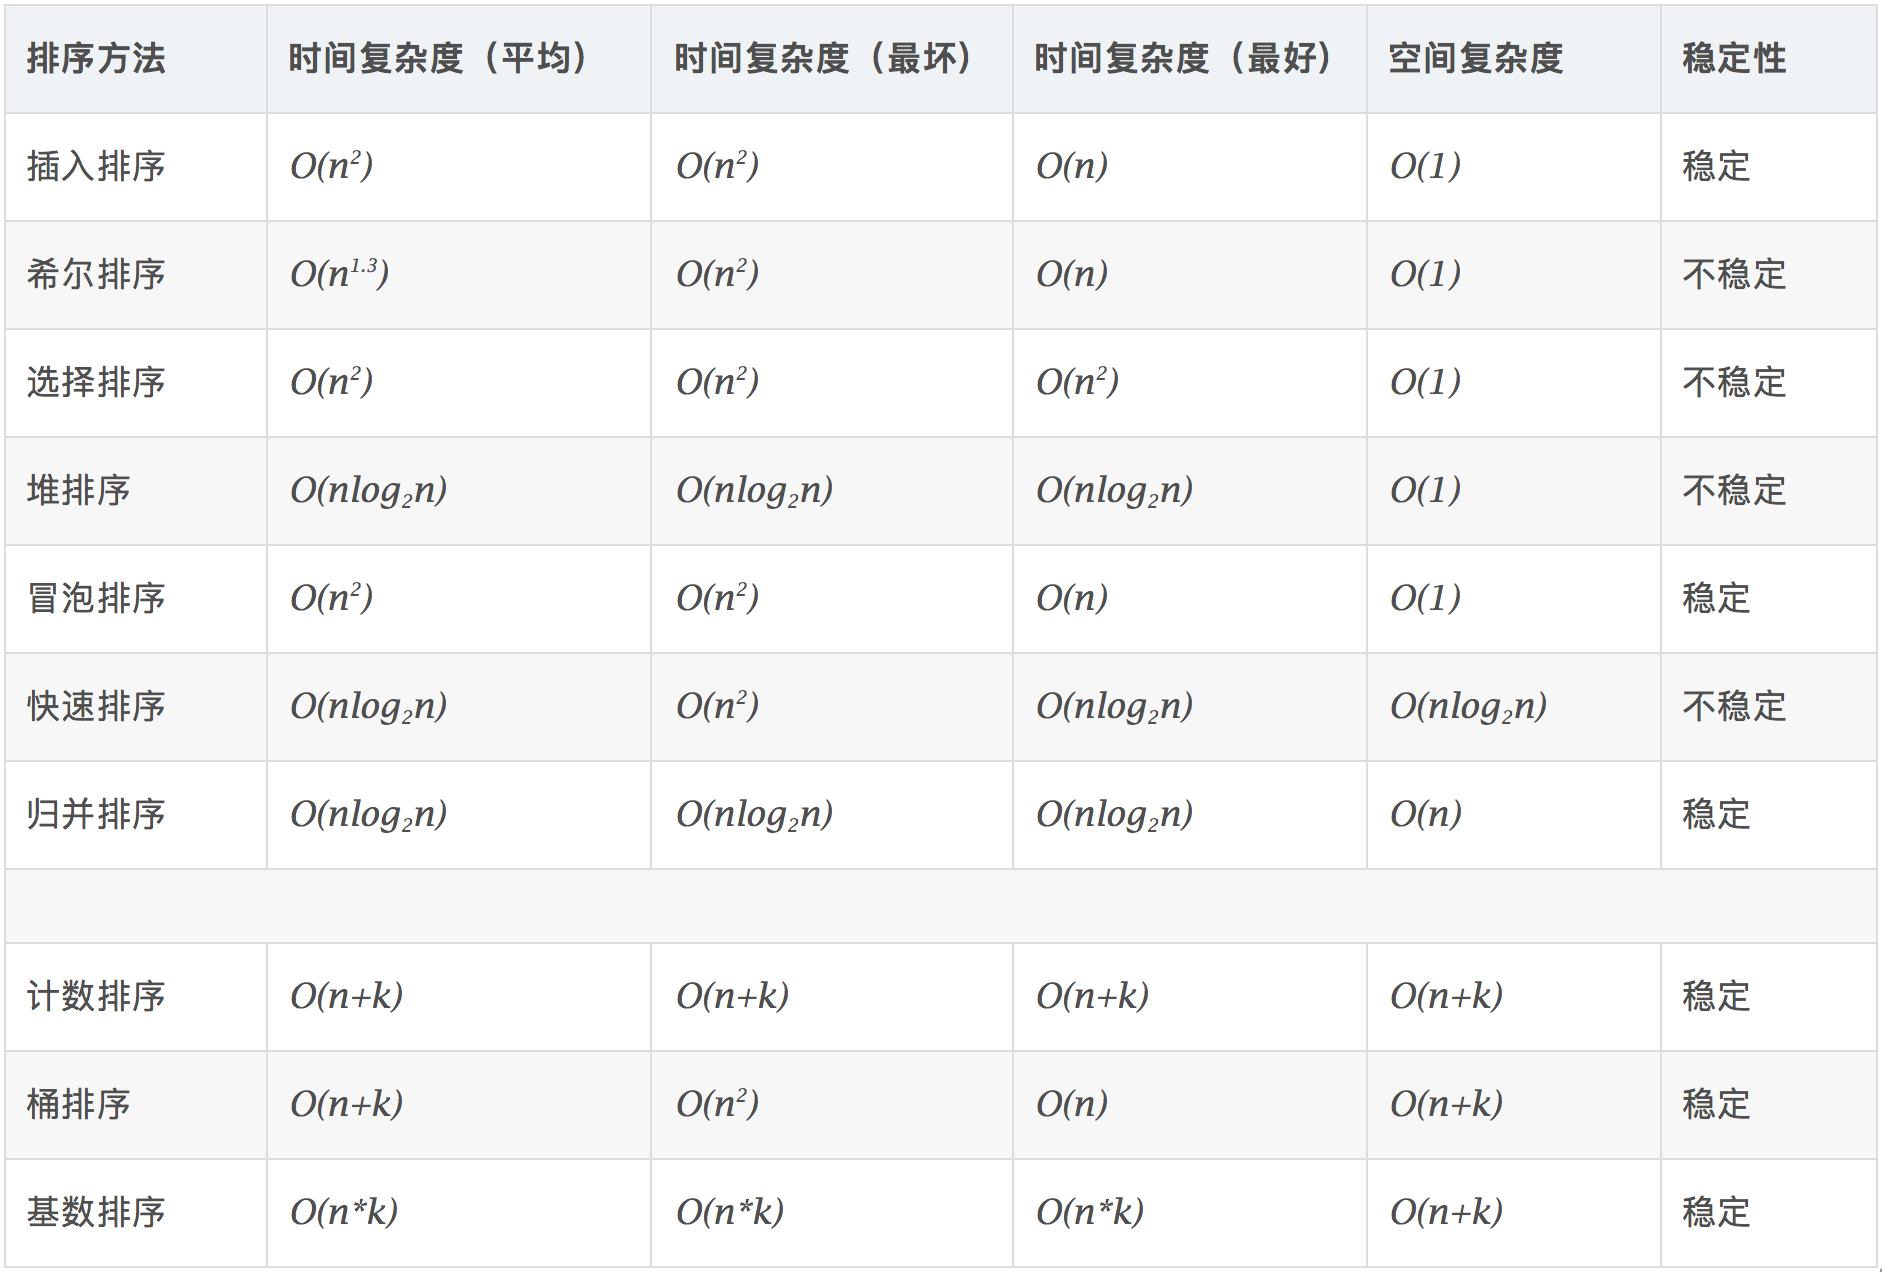
\includegraphics[width=.9\linewidth]{./pic/sort2.png}

\section{1996. The Number of Weak Characters in the Game 桶排序}
\label{sec-3-1}
You are playing a game that contains multiple characters, and each of the characters has two main properties: attack and defense. You are given a 2D integer array properties where properties[i] = [attacki, defensei] represents the properties of the ith character in the game.
A character is said to be weak if any other character has both attack and defense levels strictly greater than this character's attack and defense levels. More formally, a character i is said to be weak if there exists another character j where attackj > attacki and defensej > defensei.
Return the number of weak characters.
\begin{minted}[frame=lines,fontsize=\scriptsize,linenos=false]{java}
public int numberOfWeakCharacters(int[][] properties) {
    int maxAttrack = 0; // 找到所有士兵中的最大值
    for (int[] p : properties)
        maxAttrack = Math.max(maxAttrack,p[0]);
    // 为每一个攻击创建一个桶的位置
    int[] bucket = new int[maxAttrack + 2];     
    // 在每一个攻击力上找到最大的防御力
    for (int[] p : properties)
        bucket[p[0]] = Math.max(bucket[p[0]],p[1]);
    // 将桶的每一个位置都寻找到大于其攻击力的最大防御数值
    int rightMax = bucket[maxAttrack];
    for (int i = maxAttrack; i >= 0; i--) 
        if (rightMax > bucket[i])
            bucket[i] = rightMax;
        else
            rightMax = bucket[i];
    int ans = 0;
    // 最后遍历p 寻找所有的弱将
    for (int[] p : properties)
        if (bucket[p[0] + 1] > p[1]) ans++;  // 攻击力比当前小兵的攻击力大1的桶的位置存放着最大的防御力,与这个防御作比较可以得到当前小兵是否全面弱
    return ans;
}
public int numberOfWeakCharacters(int[][] properties) {
    int cnt = 0;
    int len = properties.length;
    Arrays.sort(properties, (a, b) -> (a[0] ! =  b[0] ? a[0]-b[0] : b[1]-a[1]));
    int max = properties[len-1][1];
    for(int i = len-1;i> = 0;i--){
        if(properties[i][1] < max)
            cnt++;
        max = Math.max(max,properties[i][1]);
    }
    return cnt;
}
\end{minted}

\section{632. Smallest Range Covering Elements from K Lists}
\label{sec-3-2}
You have k lists of sorted integers in non-decreasing order. Find the smallest range that includes at least one number from each of the k lists.
We define the range [a, b] is smaller than range [c, d] if b - a < d - c or a < c if b - a == d - c.
\begin{minted}[frame=lines,fontsize=\scriptsize,linenos=false]{java}
// 时间复杂度:O(nk \log k)O(nklogk),其中 nn 是所有列表的平均长度,kk 是列表数量。所有的指针移动的总次数最多是 nknk 次,每次从堆中取出元素和添加元素都需要更新堆,时间复杂度是 O(\log k)O(logk),因此总时间复杂度是 O(nk \log k)O(nklogk)。
// 空间复杂度:O(k)O(k),其中 kk 是列表数量。空间复杂度取决于堆的大小,堆中维护 kk 个元素。
public int[] smallestRange(List<List<Integer>> nums) {
    int n = nums.size();
    int resMin = 0, resMax = Integer.MAX_VALUE;
    int minRg = resMax - resMin;
    int max = Integer.MIN_VALUE;
    int [] next = new int [n]; // 各子链表中比当前idx位数值大的下一个数的下标,即idx+1,初始化全为0
    Queue<Integer> q = new PriorityQueue<>(new Comparator<Integer>() {
            public int compare(Integer idx1, Integer idx2) {
                return nums.get(idx1).get(next[idx1]) - nums.get(idx2).get(next[idx2]);
            }
        });
    for (int i = 0; i < n; i++) {
        q.offer(i); // 0, 1, 2, .... n-1 真神奇呀
        max = Math.max(max, nums.get(i).get(0));
    }
    int minIdx = 0, curRg = 0;
    while (true) {
        minIdx = q.poll(); // 取出的是最小值的子链表的序号,而子链表里的当前最小值所在子链表中的位置存于next[minIdx]中
        curRg = max - nums.get(minIdx).get(next[minIdx]);
        if (curRg < minRg)  {
            minRg = curRg;
            resMin = nums.get(minIdx).get(next[minIdx]);
            resMax = max;
        }
        next[minIdx]++;
        if (next[minIdx] == nums.get(minIdx).size()) break;
        q.offer(minIdx); // 加回去,但是queue里真正比较的值已经变了,变强大了。。。 // 更新最小值的替换值 
        max = Math.max(max, nums.get(minIdx).get(next[minIdx]));  // 更新最大值
    }
    return new int [] {resMin, resMax};
}
\end{minted}
\begin{itemize}
\item 另外一种解法的
\end{itemize}
\begin{minted}[frame=lines,fontsize=\scriptsize,linenos=false]{java}
// 这里的 BB 序列是什么?我们可以用一个哈希映射来表示 BB 序列—— B[i]
// B[i] 表示 ii 在哪些列表当中出现过,
// 这里哈希映射的键是一个整数,表示列表中的某个数值,
// 哈希映射的值是一个数组,这个数组里的元素代表当前的键出现在哪些列表里。
// 如果列表集合为:
// 0: [-1, 2, 3]
// 1: [1]
// 2: [1, 2]
// 3: [1, 1, 3]
// 那么可以得到这样一个哈希映射
// -1: [0]
// 1: [1, 2, 3, 3]
// 2: [0, 2]
// 3: [0, 3]
// 时间复杂度:O(nk + |V|)O(nk+∣V∣),其中 nn 是所有列表的平均长度,kk 是列表数量,|V|∣V∣ 是列表中元素的值域,在本题中 |V| \leq 2*10^5∣V∣≤2∗10 
// 5
// 。构造哈希映射的时间复杂度为 O(nk)O(nk),双指针的移动范围为 |V|∣V∣,在此过程中会对哈希映射再进行一次遍历,时间复杂度为 O(nk)O(nk),因此总时间复杂度为 O(nk + |V|)O(nk+∣V∣)。
// 空间复杂度:O(nk)O(nk),即为哈希映射使用的空间。哈希映射的「键」的数量由列表中的元素个数 nknk 以及值域 |V|∣V∣ 中的较小值决定,「值」为长度不固定的数组,但是它们的长度之和为 nknk,因此哈希映射使用的空间为 O(nk)O(nk)。在使用双指针时,还需要一个长度为 nn 的数组,其对应的空间在渐进意义下小于 O(nk)O(nk),因此可以忽略。
public int[] smallestRange(List<List<Integer>> nums) {
    int n = nums.size();
    Map<Integer, List<Integer>> indices = new HashMap<>();
    int xmin = Integer.MAX_VALUE, xmax = Integer.MIN_VALUE;
    for (int i = 0; i < n; i++) {
        for (int v : nums.get(i)) { // 把大链表中出出过的每一个值作键,值为它所存在于的子链表序号链表
            List<Integer> list = indices.getOrDefault(v, new ArrayList<>());
            list.add(i);
            indices.put(v, list);
            xmin = Math.min(xmin, v);
            xmax = Math.max(xmax, v); // 这里得到全局的最小最大值
        }
    }
    int [] freq = new int [n];
    int inside = 0; // cnt # of lists included in miniRanges
    int left = xmin, right = xmin -1;
    int resLeft = xmin, resRight = xmax;
    while (right < xmax) {
        right ++;
        if (indices.containsKey(right)) {
            for (int x : indices.get(right)) {
                freq[x]++;
                if (freq[x] == 1) inside++;
            }
            while (inside == n) { // find ONE satified solution, try to minimize the range
                if (right - left < resRight - resLeft) {
                    resLeft = left;
                    resRight = right;
                }
                if (indices.containsKey(left))  // sliding the left size towards right
                    for (int v : indices.get(left)) {
                        freq[v]--;
                        if (freq[v] == 0) --inside;
                    }
                left++;
            }
        }
    }
    return new int [] {resLeft, resRight};
}
\end{minted}

\section{Reverse Pairs}
\label{sec-3-3}
Given an integer array nums, return the number of reverse pairs in the array.
A reverse pair is a pair (i, j) where 0 <= i < j < nums.length and nums[i] > 2 * nums[j].
\begin{minted}[frame=lines,fontsize=\scriptsize,linenos=false]{java}
private int mergeSortCount(long [] arr, int bgn, int end) {
if (bgn >= end) return 0;
int mid = bgn + (end-bgn)/2;
int cnt = mergeSortCount(arr, bgn, mid) + mergeSortCount(arr, mid+1, end);
    for (int i = bgn, j = mid+1; i <= mid; i++) {
        while (j <= end && arr[i] > 2*arr[j]) j++;
        cnt += j - (mid+1);
    }
    Arrays.sort(arr, bgn, end+1);
    return cnt;
}
public int reversePairs(int[] nums) {
    int n = nums.length;
    return mergeSortCount(Arrays.stream(nums).mapToLong(i -> i).toArray(), 0, n-1);
}
// bit 的解法: https://www.cnblogs.com/grandyang/p/6657956.html
\end{minted}

\section{306. Additive Number}
\label{sec-3-4}
Additive number is a string whose digits can form additive sequence.

A valid additive sequence should contain at least three numbers. Except for the first two numbers, each subsequent number in the sequence must be the sum of the preceding two.

Given a string containing only digits '0'-'9', write a function to determine if it's an additive number.

Note: Numbers in the additive sequence cannot have leading zeros, so sequence 1, 2, 03 or 1, 02, 3 is invalid.
\begin{minted}[frame=lines,fontsize=\scriptsize,linenos=false]{java}
public boolean isAdditiveNumber(String num) {
    int n = num.length();
    if (n < 3) return false;
    for (int i = 1; i <= num.length() >> 1; i++)
        for (int j = 1; j + i < num.length(); j++)  
            if (isValid(num, num.substring(0, i), num.substring(i, i + j), i + j)) return true;
    return false;
}
private boolean isValid(String num, String first, String second, int index) {
    if (first.length() > 1 && first.startsWith("0") 
        || second.length() > 1 && second.startsWith("0")) return false;
    if (index == num.length()) return true; // 如果只有两个数是有效的!!!
    long sum = Long.parseLong(first) + Long.parseLong(second);
    if (num.startsWith(sum + "", index)) // 间接检测第三个数
        if (isValid(num, second, sum + "", index + (sum + "").length())) return true;
    return false;
}
\end{minted}


\chapter{dfs}
\label{sec-4}
\section{464. Can I Win}
\label{sec-4-1}
In the "100 game" two players take turns adding, to a running total, any integer from 1 to 10. The player who first causes the running total to reach or exceed 100 wins.
What if we change the game so that players cannot re-use integers?
For example, two players might take turns drawing from a common pool of numbers from 1 to 15 without replacement until they reach a total >= 100.
Given two integers maxChoosableInteger and desiredTotal, return true if the first player to move can force a win, otherwise, return false. Assume both players play optimally.
\begin{minted}[frame=lines,fontsize=\scriptsize,linenos=false]{java}
// state是前走的人走完之后的局面,sum是当前数字总和,返回的是当前走的人是否能赢
private boolean dfs(int max, int target, int state, int val) {
    if (dp[state] != -1) return dp[state] > 0;
    if (val >= target) { // 如果对方取数的时候总和达到target了,则当前走的人输了,做记忆并返回false
        dp[state] = 0;
        return false;
    }
    for (int i = 1; i <= max; i++) {  // 枚举当前人取哪个数
        if ((state >> i-1 & 1) == 0 && !dfs(max, target, state | (1 << i-1), val + i)) {
            dp[state] = 1;
            return true;
        }
    }
    dp[state] = 0;
    return false;
}
int [] dp;
public boolean canIWin(int maxChoosableInteger, int desiredTotal) {
    if (desiredTotal <= maxChoosableInteger) return true;
    if (desiredTotal > (maxChoosableInteger + 1)*maxChoosableInteger / 2) return false;
    dp = new int[1 << maxChoosableInteger]; // 时空复杂度O ( 2 m ) O(2^m)O(2 
    Arrays.fill(dp, -1);
    return dfs(maxChoosableInteger, desiredTotal, 0, 0);
}
\end{minted}


\chapter{排列与组合}
\label{sec-5}
\section{903. Valid Permutations for DI Sequence - Hard}
\label{sec-5-1}
You are given a string s of length n where s[i] is either:

'D' means decreasing, or
'I' means increasing.
A permutation perm of n + 1 integers of all the integers in the range [0, n] is called a valid permutation if for all valid i:

If s[i] \texttt{= 'D', then perm[i] > perm[i + 1], and
If s[i] =} 'I', then perm[i] < perm[i + 1].
Return the number of valid permutations perm. Since the answer may be large, return it modulo 109 + 7.

当是降序时,下一个数字不小于当前最后一个数字,反之是升序时,下一个数字小于当前最后一个数字,所以可以写出状态转移方程如下所示:
\begin{minted}[frame=lines,fontsize=\scriptsize,linenos=false]{java}
if (S[i-1] == 'D')    dp[i][j] += dp[i-1][k]    ( j <= k <= i-1 )
else                  dp[i][j] += dp[i-1][k]    ( 0 <= k < j )
\end{minted}
\begin{minted}[frame=lines,fontsize=\scriptsize,linenos=false]{java}
public int numPermsDISequence(String s) {
    int n = s.length(), mod = (int)1e9 + 7, res = 0;
    int [][] dp = new int [n+1][n+1];
    dp[0][0] = 1;
    for (int i = 1; i <= n; i++) 
        for (int j = 0; j <= i; j++) // 考虑当前最后一个元素为j
            if (s.charAt(i-1) == 'D')
                // 可以把序列中所有大于等于j的元素都加上1得到新序列(这个时候是不会改变当前序列的大小关系的),再把j添加到序列末尾得到
                for (int k = j; k <= i; k++) 
                    dp[i][j] = (dp[i][j] + dp[i-1][k]) % mod;
            else // 考虑当前最后一个元素为j
                // 把该序列中所有大于等于j(k < j <= i)的数字都加上1,并在末尾添加一个j得到dp[i][j]中的一种方案
                for (int k = 0; k < j; k++) // 把序列中所有大等于j的元素都加上1,再把j放在序列末尾得到
                    dp[i][j] = (dp[i][j] + dp[i-1][k]) % mod;
    for (int i = 0; i <= n; i++) 
        res = (res + dp[n][i]) % mod;
    return (int)res;
}
\end{minted}

\section{1467. Probability of a Two Boxes Having The Same Number of Distinct Balls - Hard}
\label{sec-5-2}
Given 2n balls of k distinct colors. You will be given an integer array balls of size k where balls[i] is the number of balls of color i. 

All the balls will be shuffled uniformly at random, then we will distribute the first n balls to the first box and the remaining n balls to the other box (Please read the explanation of the second example carefully).

Please note that the two boxes are considered different. For example, if we have two balls of colors a and b, and two boxes [] and (), then the distribution [a] (b) is considered different than the distribution [b] (a) (Please read the explanation of the first example carefully).

We want to calculate the probability that the two boxes have the same number of distinct balls.

Example: [2, 1, 1]

for first ball, we can put both ball in first bin and 0 ball in second bin OR we can put 1 ball in first bin, second ball in 2nd bin OR we can put both in second bin

for second ball, we can put ball in first bin and 0 ball in second bin, similarly, we can put 1 ball in second bin.

same thing with the third ball

Try all possible permutations recursively. And, in the end check, if there are equal number of distinct balls in both bins or not.

\begin{minted}[frame=lines,fontsize=\scriptsize,linenos=false]{java}
public double getProbability(int[] balls) {
    int sum = Arrays.stream(balls).sum();
    double all = allCases(balls, 0, 0, 0, 0, 0, sum);
    double valid = casesWithEqualDistinctBalls(balls, 0, 0, 0, 0, 0, sum);
    return (1.0 * valid / all);
}
// disF = distinct balls in first bin
// disS = distinct balls in second bin
// f = number of balls in first bin
// s = number of balls in second bin
public double allCases(int [] arr, int pos, int f, int s, int disF, int disS, int sum) {
    if (pos == arr.length) {
        // for all cases, we just need to check if both bins have same number of balls or not
        if (f == s) return fact(sum / 2) * fact(sum / 2); // numerator of our permutations
        return 0;
    }
    // we put all balls in second bin
    double ans = 1.0 * allCases(arr, pos+1, f, s+arr[pos], disF, disS+1, sum) / fact(arr[pos]);
    // we put all balls in first bin
    ans += 1.0 * allCases(arr, pos+1, f+arr[pos], s, disF+1, disS, sum) / fact(arr[pos]);
    for (int i = 1; i < arr[pos]; i++) // 把每一种颜色的球放到两个里面盒子里都有
        ans += 1.0 * allCases(arr, pos+1, f+i, s+arr[pos]-i, disF+1, disS+1, sum) / (fact(i) * fact(arr[pos]-i));
    return ans;
}
public double casesWithEqualDistinctBalls(int [] arr, int pos, int f, int s, int disF, int disS, int sum) {
    if (pos == arr.length) {
        if (f == s && disF == disS) return fact(sum / 2) * fact(sum / 2);
        return 0;
    }
    double ans = 1.0 * casesWithEqualDistinctBalls(arr, pos+1, f, s+arr[pos], disF, disS+1, sum) / fact(arr[pos]);
    ans += 1.0 * casesWithEqualDistinctBalls(arr, pos+1, f+arr[pos], s, disF+1, disS, sum) / fact(arr[pos]);
    for (int i = 1; i < arr[pos]; i++) 
        ans += 1.0 * casesWithEqualDistinctBalls(arr, pos+1, f+i, s+arr[pos]-i, disF+1, disS+1, sum) / (fact(i) * fact(arr[pos]-i));
    return ans;
}
private double fact(double n) {
    double res = 1;
    for (int i = 2; i <= n; i++) 
        res = res * i;
    return res;
}
// Complexity: There can be total of (8 * 6) balls with 8 distinct. Complexity of recursion is f * s * disF * disS = O(48 * 48 * 8 * 8)
\end{minted}


\chapter{Union Find 并查集}
\label{sec-6}
\section{1697. Checking Existence of Edge Length Limited Paths - Hard}
\label{sec-6-1}
An undirected graph of n nodes is defined by edgeList, where edgeList[i] = [ui, vi, disi] denotes an edge between nodes ui and vi with distance disi. Note that there may be multiple edges between two nodes.

Given an array queries, where queries[j] = [pj, qj, limitj], your task is to determine for each queries[j] whether there is a path between pj and qj such that each edge on the path has a distance strictly less than limitj .

Return a boolean array answer, where answer.length == queries.length and the jth value of answer is true if there is a path for queries[j] is true, and false otherwise.
\begin{minted}[frame=lines,fontsize=\scriptsize,linenos=false]{java}
private class DisjointSetUnion {
    private int N;
    private int [] parent, rank;
    public DisjointSetUnion( int n) {
        this.N = n;
        this.parent = new int [N];
        this.rank = new int [N];
        for (int i = 0; i < N; i++) {
            this.parent[i] = i;
            this.rank[i] = 1;
        }
    }
    public boolean areConnected(int u, int v) {
        return find(u) == find(v);
    }
    public void union(int u, int v) { // O(Log(N))
        if (u != v) {
            int p = find(u);
            int q = find(v);
            if (p != q) {
                if (rank[p] > rank[q]) {
                    parent[q] = p;
                    rank[p] += rank[q];
                } else {
                    parent[p] = q;
                    rank[q] += rank[p];
                }
            }
        }
    }
    private int find(int v) { // 我记得这里有个同步更新父数组的优化步骤,和rank优化冲突吗?要总结一下 // O(Log(N))
        int x = v;
        while (x != parent[x])
            x = parent[x];
        parent[v] = x;
        return x;
    }
}
class Query implements Comparable<Query> {
    public int idx, start, end, weight;
    public Query(int idx, int bgn, int end, int weight) {
        this.idx = idx;
        this.start = bgn;
        this.end = end;
        this.weight = weight;
    }
    @Override public int compareTo(Query query) {
        return this.weight - query.weight;
    }
}
// 我们可以分别对 edges 和 queries 进行一次升序排序。本题和 1170. 比较字符串最小字母出现频次 类似, 都可以采取 *离线排序优化* 的方式来解。
// 接下来,遍历 queries。遍历 queries 的同时将权值小于 limitj 的边进行合并。
// 接下来,我们只需要判断 pj 和 qj 是否已经在同一个联通域即可。
// 因此如果 pj 和 qj 在同一个联通域,那么其联通的路径上的所有边必定都小于 limitj,其原因就是前面加粗的那句话。
// 注意到排序打乱了 queries 的索引,因此我们需要记录一下其原始索引。
public boolean[] distanceLimitedPathsExist(int n, int[][] edgeList, int[][] queries) {
    DisjointSetUnion set = new DisjointSetUnion(n);
    Arrays.sort(edgeList, (a, b) -> a[2]-b[2]); // arrange edges in ascending order of weights
    int m = queries.length, i;
    int E = edgeList.length;
    Query [] qarr = new Query[m];
    for (i = 0; i < m; i++) 
        qarr[i] = new Query(i, queries[i][0], queries[i][1], queries[i][2]);
    Arrays.sort(qarr);                // arrange queries in ascending order of threshold weights
    boolean [] ans = new boolean [m];
    int idx = 0;
    for (i = 0; i < m; i++) {
        while (idx < E && edgeList[idx][2] < qarr[i].weight) {
            set.union(edgeList[idx][0], edgeList[idx][1]);
            ++idx;
        }
        ans[qarr[i].idx] = set.areConnected(qarr[i].start, qarr[i].end);
    }
    return ans;
}
// 令 m, q edges 和 queries 的长度。
//     时间复杂度:$O(mlogm + qlogq)
//     空间复杂度:$O(n + q)
// Runtime is bound by sorting: O(ElogE + NlogN + N + E);
\end{minted}

\section{2003. Smallest Missing Genetic Value in Each Subtree - Hard}
\label{sec-6-2}
There is a family tree rooted at 0 consisting of n nodes numbered 0 to n - 1. You are given a 0-indexed integer array parents, where parents[i] is the parent for node i. Since node 0 is the root, parents\footnote{DEFINITION NOT FOUND.} == -1.

There are 105 genetic values, each represented by an integer in the inclusive range [1, 105]. You are given a 0-indexed integer array nums, where nums[i] is a distinct genetic value for node i.

Return an array ans of length n where ans[i] is the smallest genetic value that is missing from the subtree rooted at node i.

The subtree rooted at a node x contains node x and all of its descendant nodes.
\begin{minted}[frame=lines,fontsize=\scriptsize,linenos=false]{java}
private void dfs(int i, Set<Integer> visited, int [] arr) { // 图的遍历:自顶向下ok,自底向上还不太熟悉,需要练习,还有一个没有消化好的类似题,找出来binary indexed tree
    if (!visited.contains(arr[i])) {
        Set<Integer> children = tree.getOrDefault(i, new HashSet<Integer>());
        for (int v : children) 
            dfs(v, visited, arr);
        visited.add(arr[i]);
    }
}
Map<Integer, Set<Integer>> tree = new HashMap<>();
int [] ans;
int n;
public int[] smallestMissingValueSubtree(int[] parents, int[] nums) {
    n = parents.length;
    ans = new int [n];
    Arrays.fill(ans, 1); 
    int oneIdx = -1;
    for (int i = 0; i < n; i++) 
        if (nums[i] == 1) {
            oneIdx = i;
            break;
        }
    if (oneIdx == -1) return ans;
    for (int i = 1; i < n; i++) {
        tree.computeIfAbsent(parents[i], k -> new HashSet<Integer>());
        tree.get(parents[i]).add(i);
        // tree.computeIfAbsent(i, k -> new HashSet<Integer>()); // 这里要想一下:为什么双向图他只加一个方向?
        // tree.get(i).add(parents[i]);
    }
    Set<Integer> visited = new HashSet<>(); // 这个直接转化为想要的结果,很便捷
    int parentIter = oneIdx;
    int miss = 1;
    while (parentIter >= 0) { // 从值为1的节点向根遍历(自底向上),没有任何重复计算,只走完这一条自底向项的路径就可以了
        dfs(parentIter, visited, nums);
        while (visited.contains(miss)) ++miss;
        ans[parentIter] = miss;
        parentIter = parents[parentIter];
    }
    return ans;
}
\end{minted}

\section{803. Bricks Falling When Hit - Hard 反向: 变de-Union vs为 Re-Union}
\label{sec-6-3}
You are given an m x n binary grid, where each 1 represents a brick and 0 represents an empty space. A brick is stable if:

It is directly connected to the top of the grid, or
At least one other brick in its four adjacent cells is stable.
You are also given an array hits, which is a sequence of erasures we want to apply. Each time we want to erase the brick at the location hits[i] = (rowi, coli). The brick on that location (if it exists) will disappear. Some other bricks may no longer be stable because of that erasure and will fall. Once a brick falls, it is immediately erased from the grid (i.e., it does not land on other stable bricks).

Return an array result, where each result[i] is the number of bricks that will fall after the ith erasure is applied.

Note that an erasure may refer to a location with no brick, and if it does, no bricks drop.


\includegraphics[width=.9\linewidth]{./pic/hitBricks.png}

\begin{minted}[frame=lines,fontsize=\scriptsize,linenos=false]{java}
private class UnionFind {
    int [] id; // parent
    int [] cnt;// size
    public UnionFind (int n) {
        id = new int [n];
        cnt = new int [n];
        for (int i = 0; i < n; i++) {
            id[i] = i;
            cnt[i] = 1;
        }
    }
    public int find(int i) {
        while (id[i] != i) {
            id[i] = id[id[i]];
            i = id[i];
        }
        return i;
    }
    public void union(int i, int j) {
        int rootI = find(i);
        int rootJ = find(j);
        if (rootI != rootJ) {
            id[rootI] = rootJ;
            cnt[rootJ] += cnt[rootI];
        }
    }
}
private void unionAround(int x, int y, int [][] arr, UnionFind uf) {
    for (int [] d : dirs) {
        int i = x + d[0];
        int j = y + d[1];
        if (i < 0 || i >= m || j < 0 || j >= n) continue;
        if (arr[i][j] == 1) uf.union(x*n+y+1, i*n+j+1); // +1
    }
    if (x == 0) uf.union(x*n+y+1, 0); // 第一排的直接与顶相连 // trick: to help calculate cnts connecting top easier/faster
}
int [][] dirs = {{1, 0}, {-1, 0}, {0, 1}, {0, -1}};
int m, n;
public int[] hitBricks(int[][] grid, int[][] hits) {
    m = grid.length;
    n = grid[0].length;
    for (int [] hit : hits)              // 首先把所有要打的砖块标记为2.
        if (grid[hit[0]][hit[1]] == 1)   // 如果有砖头
            grid[hit[0]][hit[1]] = 2;
    UnionFind uf = new UnionFind(m*n+1); // 这里的 + 1主要是多一个0来表示顶,所有的第一排的砖在unionfind的时候都会直接与这个0相连。
    for (int i = 0; i < m; i++)          // 然后对打掉后的数组中的砖块进行四个方向的union
        for (int j = 0; j < n; j++) 
            if (grid[i][j] == 1)
                unionAround(i, j, grid, uf);
    int cnt = uf.cnt[uf.find(0)];        // 这个count就是打完后一定会剩下的砖块数量.
    int [] ans = new int [hits.length];
    for (int i = hits.length-1; i >= 0; i--) {
        int [] hit = hits[i];
        if (grid[hit[0]][hit[1]] == 2) { // 对于需要复原的这个砖块做四个方向union,主要是为了得到有多少砖必须通过这块砖才能连接到顶部。
            unionAround(hit[0], hit[1], grid, uf);
            grid[hit[0]][hit[1]] = 1;    // 由于是从后向前,做完要把这块砖重新标记回来: 这些砖是有可能被hits前序砖敲掉后掉落下来的,不复原影响前序结果
        }
        int newCnt = uf.cnt[uf.find(0)];
        ans[i] = (newCnt - cnt > 0 ? newCnt - cnt - 1 : 0);
        cnt = newCnt;
    }
    return ans;
}
\end{minted}

\section{721. Accounts Merge}
\label{sec-6-4}
Given a list of accounts where each element accounts[i] is a list of strings, where the first element accounts[i]\footnotemark[1]{} is a name, and the rest of the elements are emails representing emails of the account.

Now, we would like to merge these accounts. Two accounts definitely belong to the same person if there is some common email to both accounts. Note that even if two accounts have the same name, they may belong to different people as people could have the same name. A person can have any number of accounts initially, but all of their accounts definitely have the same name.

After merging the accounts, return the accounts in the following format: the first element of each account is the name, and the rest of the elements are emails in sorted order. The accounts themselves can be returned in any order.

\begin{itemize}
\item Similar to the most voted solution, my solution uses the index of the owner as the key for the union map, to avoid possible issue caused by different owners have the same name, thus uses one less loop.
\end{itemize}

\begin{minted}[frame=lines,fontsize=\scriptsize,linenos=false]{java}
private int findParent(int [] arr, int x) {
    if (arr[x] == x) return x;
    arr[x] = findParent(arr, arr[x]);
    return arr[x];
}
public List<List<String>> accountsMerge(List<List<String>> accounts) {
    Map<String, Integer> owner = new HashMap<>();
    Map<Integer, TreeSet<String>> union = new HashMap<>(); // match idx & Set<Sting emails>
    int n = accounts.size(), p = 0;
    int [] par = new int [n];
    for (int i = 0; i < n; i++) par[i] = i;
    List<String> ls = new ArrayList<>(); 
    for (int i = 0; i < n; i++) { // find the ownerIdx for each email address
        ls = accounts.get(i);
        for (int j = 1; j < ls.size(); j++) {
            String email = ls.get(j);
            if (owner.containsKey(email)) {
                p = findParent(par, owner.get(email));
                par[p] = i; // union accounts that belong to the same user here by updating parent relation
            }
            owner.put(email, i);
        }
    }
     // union all emails belong to the same owner
    for (String emal : owner.keySet()) {
        int ownerIdx = findParent(par, owner.get(emal));
        TreeSet<String> set = union.getOrDefault(ownerIdx, new TreeSet<>());
        set.add(emal);
        union.put(ownerIdx, set);
    }
// Generate return result
    List<List<String>> res = new ArrayList<>();
    for (int ownerIdx : union.keySet()) {
        ls = new ArrayList<>();
        ls.add(accounts.get(ownerIdx).get(0));  // get the owner name
        ls.addAll(union.get(ownerIdx));
        res.add(ls);
    }
    return res;
}
\end{minted}

\section{1202. Smallest String With Swaps}
\label{sec-6-5}
You are given a string s, and an array of pairs of indices in the string pairs where pairs[i] = [a, b] indicates 2 indices(0-indexed) of the string.

You can swap the characters at any pair of indices in the given pairs any number of times.

Return the lexicographically smallest string that s can be changed to after using the swaps.
\begin{minted}[frame=lines,fontsize=\scriptsize,linenos=false]{java}
int [] par;
int [] rank;
int n;
public int find(int v) {
    if (v != par[v] ) 
        par[v] = find(par[v]);
    return par[v];
}
public boolean union(int i, int j) {
    int ri = find(i);
    int rj = find(j);
    if (ri == rj) return false;
    if (rank[ri] < rank[rj]) par[ri] = rj;
    else if (rank[ri] > rank[rj]) par[rj] = ri;
    else {
        par[rj] = ri;
        rank[ri] ++; // 维护rank的值
    }
    return true;
}
public String smallestStringWithSwaps(String s, List<List<Integer>> pairs) {
    int n = s.length();
    par = new int [n];
    rank = new int [n];
    List<Queue<Character>> list = new ArrayList<>(n);
    for (int i = 0; i < n; i++) {
        par[i] = i;
        list.add(new PriorityQueue<>());
    }
    Arrays.fill(rank, 1);
    pairs.forEach(p -> union(p.get(0), p.get(1))); // Perform union for each pair.
    // Add each character to the priority queue associated with its component.
    IntStream.range(0, n).forEach(index -> list.get(find(index)).add(s.charAt(index)));
    // Build the result, by removing chars from the corresponding priority queue.
    StringBuilder buffer = new StringBuilder(n);
    IntStream.range(0, n).forEachOrdered(index -> buffer.append(list.get(find(index)).remove()));
    return buffer.toString();
}
// O(NlogN). Worst-case, all indices are part of the same component. So we will essentially be popping off from the same priority queue.
// Space Complexity: O(N).
\end{minted}

\section{1998. GCD Sort of an Array - Hard}
\label{sec-6-6}
You are given an integer array nums, and you can perform the following operation any number of times on nums:

Swap the positions of two elements nums[i] and nums[j] if gcd(nums[i], nums[j]) > 1 where gcd(nums[i], nums[j]) is the greatest common divisor of nums[i] and nums[j].
Return true if it is possible to sort nums in non-decreasing order using the above swap method, or false otherwise.
\begin{minted}[frame=lines,fontsize=\scriptsize,linenos=false]{java}
private int find (int v) {
    if (!parent.containsKey(v)) {
        parent.put(v, v);
        return v;
    }
    if (parent.get(v) != v)
        parent.put(v, find(parent.get(v)));
    return parent.get(v);
}
private void union(int x, int y) {
    int rx = find(x);
    int ry = find(y);
    if (rx != ry) parent.put(rx, ry);
}
/**
   general idea (not accepted)
   we can simply union pairs of numbers which has gcd > 1 in quadratic time and then check of groups that
   are formed by union of pairs can be invidually sorted. 
   improved (accpeted)
   In above approach problem is we are union-ing pairs in quadratic time. To improve upon it. We union a number
   which is present in 'nums' with its smallest prime factor. thus if two numbers has same smallest prime factor
   their gcd is guaranted to be > 1. 
**/
Map<Integer, Integer> parent = new HashMap<>();
public boolean gcdSort(int[] arr) {
    int n = arr.length;
    parent = new HashMap<Integer, Integer>();
    int [] sorted = arr.clone();
    Arrays.sort(sorted);
    int max = Arrays.stream(arr).max().getAsInt();
    Set<Integer> numSet = new HashSet<>();
    numSet.addAll(Arrays.stream(arr).boxed().collect(Collectors.toList()));
    int p = 2;  // Seive algorithm
    boolean [] primes = new boolean [max + 1];
    Arrays.fill(primes, true);
    while (p < max) {
        if (primes[p]) {
            for (int i = p; i <= max; i += p) { // 我合并的是数组的索引,他优化成合并所有拥有公约数为p的数组中沿未合并的值
                if (numSet.contains(i)) union(p, i);
                primes[i] = false;
            }
        }
        p++;
    }
    for (int i = 0; i < n; i++) 
        if (arr[i] != sorted[i] && find(sorted[i]) != find(arr[i])) return false;
    return true;
}
\end{minted}

\section{1724 给定一个n nn个顶点的无向带权图,要求在线回答若干询问,每次询问是个三元组( p , q , x ) (p,q,x)(p,q,x),是问是否存在p pp到q qq的每条边都小于x xx的路径。}
\label{sec-6-7}

先以Kruskal算法求最小生成森林,显然对于任何p pp和q qq,它们之间所有路径中最大边最小的那条路径的最大边一定是最小生成树的某条边(如果存在路径的话)。建树完成之后,对每个连通块,以任意顶点为根,将该连通块做成一棵有根树。对于每次询问,我们只需求p pp和q qq所有到它们的最近公共祖先所经过的边的最大边权就行了。可以考虑用倍增思想(以下的内容可以参考\url{https://blog.csdn.net/qq_46105170/article/details/116217633),开两个数组f} ff和g gg,其中f [ i ] [ k ] f[i][k]f[i][k]指的是从i ii节点向上跳2 k 2$^{\text{k2}}$ 
k
 步能过走到的顶点是谁(如果跳出界了则规定值为− 1 -1−1),g [ i ] [ k ] g[i][k]g[i][k]指的是从i ii节点向上跳2 k 2$^{\text{k2}}$ 
k
 的过程中经过的边的最大权值(在不会跳出界的情况下),然后从每个树根做BFS,初始化f [ . ] [ 0 ] f[.]\footnotemark[1]{}f[.]\footnotemark[1]{}和g [ . ] [ 0 ] g[.]\footnotemark[1]{}g[.]\footnotemark[1]{}。由于在询问的时候需要知道最近公共祖先,所以还需要一个数组d dd记录每个顶点的深度,在BFS的时候可以同时求出。接下来,用倍增的思想计算f ff和g gg:
\begin{minted}[frame=lines,fontsize=\scriptsize,linenos=false]{java}
f[i][k] = f[f[i][k-1]][k-1]
g[i][k] = max{g[i][k-1],g[f[i][k-1]][k-1]}
\end{minted}
至此,所有的预处理就完成了。

接下来询问的时候,如果p pp与q qq不连通则直接返回false。否则看一下两个顶点的深度,不妨设p pp更深,则将p pp向上跳若干步,使得p pp与q qq一样深,同时用经过的边权更新答案。此时如果p = q p=qp=q,则答案已经求出,与x xx比较即可;否则,将p pp与q qq继续向上跳,一路跳到它们的最近公共祖先的孩子的那层位置,一路更新答案,最后再用最近公共祖先与它们的连边更新答案,最后将答案与x xx比较。代码如下:
\begin{minted}[frame=lines,fontsize=\scriptsize,linenos=false]{java}
public class DistanceLimitedPathsExist {
    class UnionFind {
        private int[] p;
        public UnionFind(int size) {
            p = new int[size];
            for (int i = 0; i < size; i++) 
                p[i] = i;
        }
        public int find(int x) {
            if (p[x] != x) 
                p[x] = find(p[x]);
            return p[x];
        }
        public void union(int x, int y) {
            int px = find(x), py = find(y);
            if (px != py) 
                p[px] = py;
        }
    }
    private UnionFind uf;
    // 这里是链式前向星建图
    private int[] h, e, ne, w;
    private int idx;
    private void add(int a, int b, int c) {
        e[idx] = b;
        ne[idx] = h[a];
        w[idx] = c;
        h[a] = idx++;
    }
    // 这里是倍增法所需的数组和变量
    private int[][] f, g;
    private int[] depth;
    // n是顶点数,log是n对2的对数,log + 1也是f的第二维应该开的长度
    private int n, log;
    public DistanceLimitedPathsExist(int n, int[][] edgeList) {
        this.n = n;
        depth = new int[n];
        h = new int[n];
        Arrays.fill(h, -1);
        // 无向图,边要开两倍
        e = new int[n << 1];
        ne = new int[n << 1];
        w = new int[n << 1];
        // 这一段是Kruskal算法建最小生成森林
        Arrays.sort(edgeList, (e1, e2) -> Integer.compare(e1[2], e2[2]));
        uf = new UnionFind(n);
        for (int[] e : edgeList) {
            int a = e[0], b = e[1], len = e[2];
            if (uf.find(a) != uf.find(b)) {
                uf.union(a, b);
                add(a, b, len);
                add(b, a, len);
            }
        }
        log = (int) (Math.log(n) / Math.log(2));
        f = new int[n][log + 1];
        g = new int[n][log + 1];
        for (int[] row : f) {
            Arrays.fill(row, -1);
        }
        boolean[] vis = new boolean[n];
        for (int i = 0; i < n; i++) {
            if (!vis[i]) {
                bfs(i, vis);
            }
        }
        init();
    }
    // 递推一遍f和g数组
    private void init() {
        for (int i = 1; i < log + 1; i++) {
            for (int j = 0; j < n; j++) {
                if (f[j][i - 1] != -1) {
                    f[j][i] = f[f[j][i - 1]][i - 1];
                    g[j][i] = Math.max(g[j][i - 1], g[f[j][i - 1]][i - 1]);
                }
            }
        }
    }
    // BFS一遍x所在连通块,并初始化f和g数组,并求出depth数组
    private void bfs(int x, boolean[] vis) {
        Queue<Integer> q = new ArrayDeque<>();
        q.offer(x);
        vis[x] = true;
        while (!q.isEmpty()) {
            int u = q.poll();
            for (int i = h[u]; i != -1; i = ne[i]) {
                int v = e[i];
                if (vis[v]) continue;
                vis[v] = true;
                f[v][0] = u;
                g[v][0] = w[i];
                q.offer(v);
                depth[v] = depth[u] + 1;
            }
        }
    }
    public boolean query(int p, int q, int limit) {
        if (uf.find(p) != uf.find(q)) 
            return false;
        if (depth[p] < depth[q]) {
            int tmp = p;
            p = q;
            q = tmp;
        }
        // 先走到同一深度
        int diff = depth[p] - depth[q];
        int pow = 0, max = 0;
        while (diff > 0) {
            if ((diff & 1) == 1) {
                max = Math.max(max, g[p][pow]);
                p = f[p][pow];
            }

            pow++;
            diff >>= 1;
        }
        // 已经走到同一点了,那深度更浅的那个点就是最近公共祖先,max就是经过的边的最大值
        if (p == q) return max < limit;
        // 否则跳到最近公共祖先下面一层,沿途更新答案
        for (int i = log; i >= 0; i--) {
            if (f[p][i] != f[q][i]) {
                max = Math.max(max, g[p][i]);
                max = Math.max(max, g[q][i]);
                p = f[p][i];
                q = f[q][i];
            }
        }
        // 最后别忘了用最后一步更新答案
        max = Math.max(max, g[p][0]);
        max = Math.max(max, g[q][0]);
        return max < limit;
    }
}
// 初始化时间复杂度O ( m log ⁡ m + n log ⁡ n ) O(m\log m+n\log n)O(mlogm+nlogn),每次询问时间O ( log ⁡ n ) O(\log n)O(logn),空间O ( m + n + n log ⁡ n ) O(m+n+n\log n)O(m+n+nlogn)。
\end{minted}

\section{1172. 祖孙询问}
\label{sec-6-8}
给定一棵包含n nn个节点的有根无向树,节点编号互不相同,但不一定是1 ∼ n 1∼n1∼n。有m mm个询问,每个询问给出了一对节点的编号x xx和y yy,询问x xx与y yy的祖孙关系。

输入格式:
输入第一行包括一个整数 表示节点个数;接下来n nn行每行一对整数a aa和b bb,表示a aa和b bb之间有一条无向边。如果b bb是− 1 −1−1,那么a aa就是树的根;第n + 2 n+2n+2行是一个整数m mm表示询问个数;接下来m mm行,每行两个不同的正整数x xx和y yy,表示一个询问。

输出格式:
对于每一个询问,若x xx是y yy的祖先则输出1 11,若y yy是x xx的祖先则输出2 22,否则输出0 00。

数据范围:
1 ≤ n , m ≤ 4 × 1 0 4 1≤n,m≤4×10$^{\text{41≤n}}$,m≤4×10 
4

1 ≤ v ≤ 4 × 1 0 4 1≤v≤4×10$^{\text{41≤v≤4×10}}$ 
4
 ,v vv是顶点编号

可以用倍增的思想来求。预处理两个数组,一个是d [ i ] d[i]d[i],指的是顶点i ii的深度,树根深度是1 11,其余顶点的深度就是其与树根的路径边数;另一个是f [ i ] [ k ] f[i][k]f[i][k],是从顶点i ii向树根方向(以下均称“向上”)跳2 k 2$^{\text{k2}}$ 
k
 步走到的顶点。由于顶点编号都是大于0 00的,我们可以人为规定一个0 00号节点作为哨兵,并且∀ k , f [ r ] [ k ] = 0 $\forall$ k,f[r][k]=0∀k,f[r][k]=0,d [ 0 ] = 0 d\footnotemark[1]{}=0d\footnotemark[1]{}=0,其中r rr是树根编号。这样如果k kk太大导致跳出树根的话,就会得到跳到了哨兵的结论。那么对于f ff,有f [ i ] [ 0 ] = p i f[i]\footnotemark[1]{}=p$_{\text{if[i]}\footnotemark[1]{}}$= 是i ii的父亲,并且:

f[i][k]=f[f[i][k−1]][k−1]

即分两次跳,一次跳2$^{\text{k}}$ 步等价于两次跳2$^{\text{k}}$-1 步。初始化f ff和d dd数组的过程,可以用一次从树根的BFS来做到。

在询问的时候,比如询问a aa和b bb的公共祖先,不妨设a aa的深度更深,那么先让a aa向上跳到与b bb深度相同,可以先计算一下d [ a ] − d [ b ] d[a]-d[b]d[a]−d[b],然后将这个数字做二进制分解,就可以由f ff数组算出从a aa向上走到与b bb深度相同的时候是哪个顶点;接着再从a aa和b bb一起向上走,直到走到它们真正的最近公共祖先的下一层为止(即跳的步数是当前深度差减1 11),此时f [ a ] [ 0 ] f[a]\footnotemark[1]{}f[a]\footnotemark[1]{}即为最近公共祖先。代码如下:
\begin{minted}[frame=lines,fontsize=\scriptsize,linenos=false]{c++}
const int N = 40010, M = N * 2;
int n, m;
int h[N], e[M], ne[M], idx;
int depth[N], fa[N][16];
int q[N];
void add(int a, int b) {
    e[idx] = b, ne[idx] = h[a], h[a] = idx++;
}
// 从树根开始bfs,预处理出d数组和f数组
void bfs(int root) {
    memset(depth, 0x3f, sizeof depth);
    depth[0] = 0, depth[root] = 1;
    int hh = 0, tt = 0;
    q[tt++] = root;
    while (hh < tt) {
        int t = q[hh++];
        for (int i = h[t]; ~i; i = ne[i]) {
            int j = e[i];
            if (depth[j] > depth[t] + 1) {
                depth[j] = depth[t] + 1;
                q[tt++] = j;
                // 预处理f数组
                fa[j][0] = t;
                for (int k = 1; k <= 15; k++) 
                    fa[j][k] = fa[fa[j][k - 1]][k - 1];
            }
        }
    }
}
int lca(int a, int b) {
	// 强制让a的深度大于等于b的深度
    if (depth[a] < depth[b]) swap(a, b);
    // 从大到小枚举k,将a向上跳到与b同层
    for (int k = 15; k >= 0; k--)
        if (depth[fa[a][k]] >= depth[b]) 
            a = fa[a][k];
	// 如果a和b重合了,那么说明b就是最近公共祖先
    if (a == b) return b;
    // 否则将a和b同时向上跳,直到跳到最近公共祖先下一层为止
    for (int k = 15; k >= 0; k--)
        if (fa[a][k] != fa[b][k])
            a = fa[a][k], b = fa[b][k];
    return fa[a][0];
}
int main() {
    scanf("%d", &n);
    memset(h, -1, sizeof h);
    int root = 0;
    for (int i = 0; i < n; i++) {
        int a, b;
        scanf("%d%d", &a, &b);
        if (b == -1) root = a;
        else add(a, b), add(b, a);
    }
    bfs(root);
    scanf("%d", &m);
    while (m--) {
        int a, b;
        scanf("%d%d", &a, &b);
        int p = lca(a, b);
        if (p == a) puts("1");
        else if (p == b) puts("2");
        else puts("0");
    }
    return 0;
}
\end{minted}


\section{某个网友列的相关题目: 并查集参考:数据结构–并查集(Disjoint-Set)}
\label{sec-6-9}
\begin{itemize}
\item 261. 以图判树(全部连通+边数=V-1)
\item 305. 岛屿数量 II(并查集)
\item 323. 无向图中连通分量的数目(并查集)
\item 684. 冗余连接(并查集)
\item 685. 冗余连接 II(并查集)
\item 721. 账户合并(并查集)(字符串合并)
\item 737. 句子相似性 II(并查集)
\item 886. 可能的二分法(着色DFS/BFS/拓展并查集)
\item 947. 移除最多的同行或同列石头(并查集)
\item 990. 等式方程的可满足性(并查集)
\item 959. 由斜杠划分区域(并查集)
\item 1061. 按字典序排列最小的等效字符串(并查集)
\item 1101. 彼此熟识的最早时间(排序+并查集)
\item 1202. 交换字符串中的元素(并查集)
\item 1319. 连通网络的操作次数(BFS/DFS/并查集)
\item 5510. 保证图可完全遍历(并查集)
\item 程序员面试金典 - 面试题 17.07. 婴儿名字(并查集)
\end{itemize}


\chapter{Graph}
\label{sec-7}
\section{2045. Second Minimum Time to Reach Destination - Hard}
\label{sec-7-1}
A city is represented as a bi-directional connected graph with n vertices where each vertex is labeled from 1 to n (inclusive). The edges in the graph are represented as a 2D integer array edges, where each edges[i] = [ui, vi] denotes a bi-directional edge between vertex ui and vertex vi. Every vertex pair is connected by at most one edge, and no vertex has an edge to itself. The time taken to traverse any edge is time minutes.

Each vertex has a traffic signal which changes its color from green to red and vice versa every change minutes. All signals change at the same time. You can enter a vertex at any time, but can leave a vertex only when the signal is green. You cannot wait at a vertex if the signal is green.

The second minimum value is defined as the smallest value strictly larger than the minimum value.

For example the second minimum value of [2, 3, 4] is 3, and the second minimum value of [2, 2, 4] is 4.
Given n, edges, time, and change, return the second minimum time it will take to go from vertex 1 to vertex n.

Notes:

You can go through any vertex any number of times, including 1 and n.
You can assume that when the journey starts, all signals have just turned green.

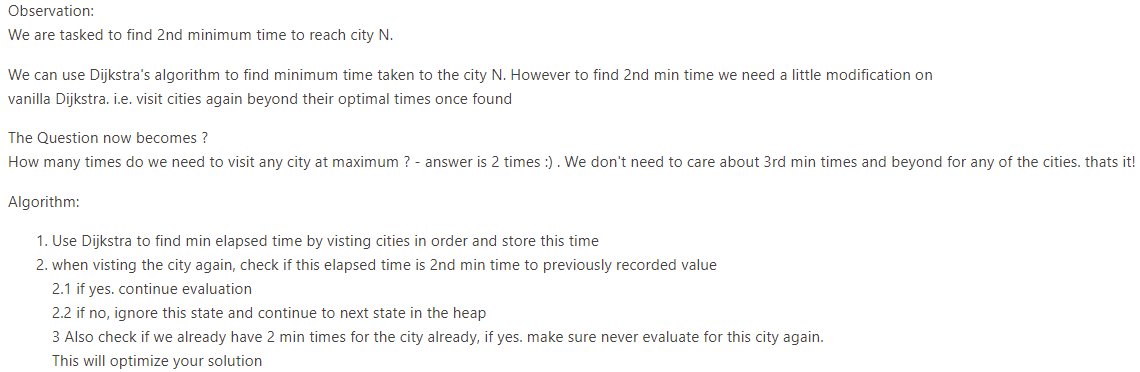
\includegraphics[width=.9\linewidth]{./pic/redGreen.png}

\begin{minted}[frame=lines,fontsize=\scriptsize,linenos=false]{java}
public int secondMinimum(int n, int[][] edges, int time, int change) {
    Map<Integer, List<Integer>> adj = new HashMap<>();
    for (int [] e : edges) {
        adj.computeIfAbsent(e[0], z -> new ArrayList<>()).add(e[1]);
        adj.computeIfAbsent(e[1], z -> new ArrayList<>()).add(e[0]);
    }
    Queue<int []> q = new PriorityQueue<>((a, b)->(a[1] -b[1]));
    q.offer(new int []{1, 0});
    Map<Integer, Integer> cache = new HashMap<>(); // use cache to record min time per city
    // modification: we want to visit each city maximum two times with different times,
    // this will help in early termination when we visit the city again (3rd time or more)
    Set<Integer> exhausted = new HashSet<>();
    while (!q.isEmpty()) {
        int [] top = q.poll();
        int cur = top[0], t = top[1];
        // Base Termination : we have found our 2nd min time for city n
        if (cur == n && t > cache.getOrDefault(cur, Integer.MAX_VALUE))
            return t;
        if (!cache.containsKey(cur)) // we vistied this city for first time, so elapsed time is min for this city
            cache.put(cur, t);
        // early termination, if we are trying to visit the city 3rd time or more ,
        // or the elapsed time will not help in finding the solution
        else if (cache.get(cur) == t || exhausted.contains(cur)) continue;
        else // this means we are visiting the city with 2nd optimal time , we dont need to visit the city ever again
            exhausted.add(cur);
        // we visit the city on elapsedTime, we need to check if on basis of change time, whether this time falls in  cycle (green or red)
        // if odd cycle (red), we must wait for this cycle to end
        int factor = t / change;
        if (factor % 2 == 1)
            t = (factor + 1) * change;
        for (int nb : adj.getOrDefault(cur, new ArrayList<>())) { // visit the neighbours
            int visTime = t + time;
            if (!exhausted.contains(nb))
                q.offer(new int [] {nb, visTime});
        }
    }
    return -1;
}
\end{minted}
\begin{itemize}
\item 另一个也是写得直接了当的
\end{itemize}
\begin{minted}[frame=lines,fontsize=\scriptsize,linenos=false]{java}
public int secondMinimum(int n, int [][] edges, int time, int change) {
    Map<Integer, Set<Integer>> map = new HashMap<>();
    for (int [] e : edges) {
        map.computeIfAbsent(e[0], z -> new HashSet<>()).add(e[1]);
        map.computeIfAbsent(e[1], z -> new HashSet<>()).add(e[0]);
    }
    Queue<int []> q = new PriorityQueue<>((a, b)->(a[1]-b[1]));
    Map<Integer, Set<Integer>> vis = new HashMap<>();
    q.offer(new int [] {1, 0});
    int min = -1;
    while (!q.isEmpty()) {
        int [] top = q.poll();
        int cur = top[0], t = top[1];
        if (cur == n) {
            if (min == -1 || min == t) min = t;
            else return t;
        }
        if (t % (2 * change) >= change)
            t += 2 * change - t % (2 * change);
        // 源码中传入key和value,根据key获取看是否存在value,如果value==null,然后调用put方法把传入的key和value  put进map,返回根据key获取的老value
        // 如果传入key对应的value已经存在,就返回存在的value,不进行替换。如果不存在,就添加key和value,返回null
        vis.putIfAbsent(cur, new HashSet<>());
        if (!vis.get(cur).add(t) || vis.get(cur).size() >= 3) continue;
        if (map.containsKey(cur))
            for (int next : map.get(cur)) 
                q.offer(new int [] {next, t + time});
    }
    return -1;
}
\end{minted}
昨天晚上的比赛,状态相对早上要差了很多,感觉到晚上的头脑已经不是很清醒。比赛的时候没有感觉,白白折腾了一个小时。
结束后去看别人题解的时候,弱弱的内心是奔溃的:
应该说这些考点平时自己也都练习过,没有过偏的地方,可为什么自己做题的时候,一个个考点穿上马甲我就再也认不出它们来了呢?
把可以重复遍历当作是多余的,不想去重复遍历;又被n迷惑住,全然忘记其它node也会被重复遍历到;明明知道pq里还有一堆杂物,比赛时却浑然想不到我是可以去裁枝优化的?!!!
昨天晚上的比赛应该是最近几周参加比赛以来做得相对较好的一次,可相比于早上最后一道题完全没有时间做、几乎没有下笔思路,这个最后一题留有整整一个小时,考点也都练习到过,却探肩而过、失之交臂、被自己活活折腾死。。。感触很多。。。。。。或许这也是一个磨砺心志、相定信念的过程吧?!!!练习练习练习、总结总结总结,让它们深入骨髓,一看便知似曾相识?

\section{1334. Floyd算法 - Find the City With the Smallest Number of Neighbors at a Threshold Distance - Medium}
\label{sec-7-2}
There are n cities numbered from 0 to n-1. Given the array edges where edges[i] = [fromi, toi, weighti] represents a bidirectional and weighted edge between cities fromi and toi, and given the integer distanceThreshold.

Return the city with the smallest number of cities that are reachable through some path and whose distance is at most distanceThreshold, If there are multiple such cities, return the city with the greatest number.

Notice that the distance of a path connecting cities i and j is equal to the sum of the edges' weights along that path.
\begin{minted}[frame=lines,fontsize=\scriptsize,linenos=false]{java}
public int findTheCity(int n, int[][] edges, int distanceThreshold) {
    // 1.创建邻接矩阵
    int [][] graph = new int [n][n]; // 相比于我只会用HashMap来建邻接关系,邻接链表与数组都可能,看哪个用起来方便
    for (int i = 0; i < n; i++)
        Arrays.fill(graph[i], Integer.MAX_VALUE); // pre filled n equaivlent to Integer.MAX_VALUE
    for (int [] eg : edges) {
        graph[eg[0]][eg[1]] = eg[2];
        graph[eg[1]][eg[0]] = eg[2];
    }
    // 2.floyd算法
    for (int k = 0; k < n; k++)          // 中间结点
        for (int i = 0; i < n; i++)      // 开始结点
            for (int j = 0; j < n; j++) {// 结尾结点
                if (i == j || graph[i][k] == Integer.MAX_VALUE || graph[k][j] == Integer.MAX_VALUE) continue;
                graph[i][j] = Math.min(graph[i][j], graph[i][k] + graph[k][j]);
            }                
    // 3.每个城市距离不大于distanceThreshold的邻居城市的数目
    int [] mark = new int [n]; //记录小于distanceThreshold的邻居城市个数
    for (int i = 0; i < n; i++) 
        for (int j = 0; j < n; j++) 
            if (graph[i][j] <= distanceThreshold)
                mark[i]++;
    // 4.找数目少,编号最大的
    int min = n;
    int ans = 0;
    for (int i = 0; i < n; i++) 
        if (min >= mark[i]) {
            min = mark[i];
            ans = i;
        }
    return ans;
}
\end{minted}
\begin{itemize}
\item 另一种解法
\end{itemize}
\begin{minted}[frame=lines,fontsize=\scriptsize,linenos=false]{java}
// 之前用原创想法也写了很多图的题,但缺乏归纳总结,原创想法更多的是解决了题目,但解法与效率、与优化算法间的距离还需要很多比较归纳与总结,才能把图这一块吃透
// https://leetcode.jp/leetcode-1334-find-the-city-with-the-smallest-number-of-neighbors-at-a-threshold-distance-%E8%A7%A3%E9%A2%98%E6%80%9D%E8%B7%AF%E5%88%86%E6%9E%90/  这个题需要重新写
// map:图结构
// city:当前城市
// dis:当前所剩距离
// v:已经被记录为邻居的节点
// maxDis:走到某个节点时,剩余距离的最大值
// 返回值为当前城市的邻居数。
private int dfs(int [][] arr, int city, int dis, boolean [] vis, int [] maxDis) {
    int res = 0;
    for (int i = 0; i < arr[0].length; i++) { // 循环当前城市的所有相邻城市
        int distance = arr[city][i]; // 与相邻城市的距离,如果为0,说明与该城市不相连
        int diffDis = dis - distance;// 到达相邻城市后,与阈值相比的剩余距离。
        if (distance > 0 && diffDis >= maxDis[i]) { // 与该城市相连并且剩余距离大于等于访问数组中的值
            maxDis[i] = diffDis;     // 更新访问数组中的剩余距离   
            if (!vis[i]) {
                vis[i] = true;
                res++;
            }
            res += dfs(arr, i, diffDis, vis, maxDis); // 递归dfs与该城市相连的其他城市:图中我似乎还很没有dfs以及递归的概念
        }
    }
    return res;
}
public int findTheCity(int n, int[][] edges, int distanceThreshold) {
    int [][] map = new int [n][n];
    for (int [] eg : edges) {
        map[eg[0]][eg[1]] = eg[2];
        map[eg[1]][eg[0]] = eg[2];
    }
    int min = n;
    int res = 0;
    for (int i = 0; i < n; i++) {
        boolean [] vis = new boolean [n];
        vis[i] = true;
        int cnt = dfs(map, i, distanceThreshold, vis, new int [n]);
        if (cnt <= min) {
            min = cnt;
            res = i;
        }
    }
    return res;
}
\end{minted}

\section{1129. Shortest Path with Alternating Colors - Medium}
\label{sec-7-3}
Consider a directed graph, with nodes labelled 0, 1, \ldots{}, n-1.  In this graph, each edge is either red or blue, and there could be self-edges or parallel edges.

Each [i, j] in red$_{\text{edges}}$ denotes a red directed edge from node i to node j.  Similarly, each [i, j] in blue$_{\text{edges}}$ denotes a blue directed edge from node i to node j.

Return an array answer of length n, where each answer[X] is the length of the shortest path from node 0 to node X such that the edge colors alternate along the path (or -1 if such a path doesn't exist).
\begin{minted}[frame=lines,fontsize=\scriptsize,linenos=false]{java}
// 找最短路径应该用queue来做,入队列的时候需要标记红边或是蓝边以便找交替路径
public int[] shortestAlternatingPaths(int n, int[][] red_edges, int[][] blue_edges) {
    HashMap<Integer, List<Integer>> [] maps = new HashMap [2]; // 0 : red; 1: blue
    for (int i = 0; i < 2; i++) 
        maps[i] = new HashMap<>();
    for (int i = 0; i < red_edges.length; i++) 
        maps[0].computeIfAbsent(red_edges[i][0], k->new ArrayList<>()).add(red_edges[i][1]);
    for (int i = 0; i < blue_edges.length; i++) 
        maps[1].computeIfAbsent(blue_edges[i][0], k->new ArrayList<>()).add(blue_edges[i][1]);
    int [] ans = new int[n];
    Arrays.fill(ans, -1);
    Queue<int []> q = new LinkedList<>();
    q.offer(new int [] {0, 0}); // red edge         
    q.offer(new int [] {0, 1}); // blue edge
    boolean [][] inQueue = new boolean [n][2]; // 0: red, 1: blue
    inQueue[0][0] = true;
    inQueue[0][1] = true;
    int cnt = 0, color = 0;
    while (!q.isEmpty()) {
        for (int size = q.size(); size > 0; size--) {
            int [] cur = q.poll();
            System.out.println(Arrays.toString(cur));
            color = cur[1];
            if (ans[cur[0]] == -1) ans[cur[0]] = cnt;
            List<Integer> nextNodes = maps[1-color].get(cur[0]);
            if (nextNodes == null) continue;
            for (Integer next : nextNodes) 
                if (!inQueue[next][1-color]) {
                    q.offer(new int [] {next, 1-color});
                    inQueue[next][1-color] = true;
                }
        }
        ++cnt;
    }
    return ans;
}
\end{minted}
\begin{itemize}
\item 不是总喜欢省掉大括号吗,试试省掉下面的。。。。。。
\end{itemize}
\begin{minted}[frame=lines,fontsize=\scriptsize,linenos=false]{java}
public int[] shortestAlternatingPaths(int n, int[][] red_edges, int[][] blue_edges) {
    int [][] red = new int[n][2]; // 红 0 蓝 1
    int [][] blue = new int[n][2];
    for (int i = 1; i < n; i++) {
        red[i][0] = i;
        red[i][1] = 0x0fffffff;   // 初始化红边权值
    }
    red [0][0] = 0;
    red [0][1] = 0;
    for (int i = 1; i < n; i++) {
        blue[i][0] = i;
        blue[i][1] = 0x0fffffff;
    }
    blue [0][0] = 0;
    blue [0][1] = 0;
    dfs(red, blue, 0, 0, red_edges, blue_edges);
    dfs(red, blue, 1, 0, red_edges, blue_edges);
    int [] ans = new int[n];
    for(int i = 0; i < n; i++){
        ans[i] = Math.min(red[i][1], blue[i][1]);
        if (ans[i] == 0x0fffffff) // 没有改变说明不存在
            ans[i] = -1;
    }
    return ans;
}
public void dfs(int [][] red, int [][] blue, int color, int node, int[][] red_edges, int[][] blue_edges){
    if (color == 0) { // 这个括号可以省吗???
        for (int [] blue_to : blue_edges) // 以node为from to 为终 的边
            if (node == blue_to[0] && red[node][1]+1 < blue[blue_to[1]][1]) {// 0到from点加1是否小于0到to的距离
                blue[blue_to[1]][1] = red[node][1]+1; // 作距离的更新
                dfs(red, blue, 1-color, blue_to[1], red_edges, blue_edges);
            }
    } else for (int [] red_to : red_edges) //以node为from to 为终 的边
               if (node == red_to[0] && blue[node][1]+1 < red[red_to[1]][1]) {//0到from点加1是否小于0到to的距离
                   red[red_to[1]][1] = blue[node][1]+1;
                   dfs(red, blue, 1-color, red_to[1], red_edges, blue_edges);
               }
}
\end{minted}

\section{882. Reachable Nodes In Subdivided Graph - Hard}
\label{sec-7-4}
You are given an undirected graph (the "original graph") with n nodes labeled from 0 to n - 1. You decide to subdivide each edge in the graph into a chain of nodes, with the number of new nodes varying between each edge.

The graph is given as a 2D array of edges where edges[i] = [ui, vi, cnti] indicates that there is an edge between nodes ui and vi in the original graph, and cnti is the total number of new nodes that you will subdivide the edge into. Note that cnti == 0 means you will not subdivide the edge.

To subdivide the edge [ui, vi], replace it with (cnti + 1) new edges and cnti new nodes. The new nodes are x1, x2, \ldots{}, xcnti, and the new edges are [ui, x1], [x1, x2], [x2, x3], \ldots{}, [xcnti-1, xcnti], [xcnti, vi].

In this new graph, you want to know how many nodes are reachable from the node 0, where a node is reachable if the distance is maxMoves or less.

Given the original graph and maxMoves, return the number of nodes that are reachable from node 0 in the new graph.

再进一步来分析,其实上对于每个结点来说(不论有没有编号),若我们能算出该结点离起始结点的最短距离,且该距离小于等于M的话,那这个结点就一定可以到达。这样来说,其实本质就是求单源点的最短距离,此时就要祭出神器迪杰斯特拉算法 Dijkstra Algorithm 了,LeetCode 中使用了该算法的题目还有 Network Delay Time 和 The Maze II。该算法的一般形式是用一个最小堆来保存到源点的最小距离,这里我们直接统计到源点的最小距离不是很方便,可以使用一个小 trick,即用一个最大堆来统计当前结点所剩的最大步数,因为剩的步数越多,说明距离源点距离越小。由于 Dijkstra 算法是以起点为中心,向外层层扩展,直到扩展到终点为止。根据这特性,用 BFS 来实现时再好不过了,首先来建立邻接链表,这里可以使用一个 NxN 的二维数组 graph,其中 graph[i][j] 表示从大结点i往大结点j方向会经过的小结点个数,建立邻接链表的时候对于每个 edge,要把两个方向都赋值,前面解释过了这里要当作有向图来做。然后使用一个最大堆,里面放剩余步数和结点编号组成的数对儿,把剩余步数放前面就可以默认按步数从大到小排序了,初始化时把 \{M,0\} 存入最大堆。还需要一个一维数组 visited 来记录某个结点是否访问过。

\begin{minted}[frame=lines,fontsize=\scriptsize,linenos=false]{java}
public int reachableNodes(int[][] edges, int maxMoves, int n) {
    int [][] graph = new int  [n][n];
    for (int i = 0; i < n; i++) 
        Arrays.fill(graph[i], -1);
    for (int [] v : edges) {
        graph[v[0]][v[1]] = v[2];
        graph[v[1]][v[0]] = v[2];
    }
    Queue<int []> q = new PriorityQueue<>((a, b) -> (b[0] - a[0]));
    boolean [] vis = new boolean [n];
    q.offer(new int [] {maxMoves, 0});
    int res = 0;
    while (!q.isEmpty()) {
        int [] cur = q.poll();
        int cnt = cur[0], u = cur[1];
        if (vis[u]) continue;
        vis[u] = true;
        ++res;
        for (int i = 0; i < n; i++) {
            if (graph[u][i] == -1) continue;
            if (cnt > graph[u][i] && !vis[i])
                q.offer(new int [] {cnt - graph[u][i]-1, i});
            graph[i][u] -= Math.min(cnt, graph[u][i]);
            res += Math.min(cnt, graph[u][i]);
        }
    }
    return res;
}
\end{minted}
\begin{itemize}
\item 我们也可以使用 HashMap 来建立邻接链表,最后的运行速度果然要比二维数组形式的邻接链表要快一些,其他的地方都不变,参见代码如下:
\end{itemize}
\begin{minted}[frame=lines,fontsize=\scriptsize,linenos=false]{java}
public int reachableNodes(int[][] edges, int maxMoves, int n) {
    int res = 0;
    Map<Integer, Map<Integer, Integer>> graph = new HashMap<>();
    for (int [] v : edges) {
        graph.computeIfAbsent(v[0], k->new HashMap<>()).put(v[1], v[2]);
        graph.computeIfAbsent(v[1], k->new HashMap<>()).put(v[0], v[2]);
    }
    Queue<int []> q = new PriorityQueue<>((a, b) -> (b[0] - a[0]));
    boolean [] vis = new boolean [n];
    q.offer(new int [] {maxMoves, 0});
    while (!q.isEmpty()) {
        int [] cur = q.poll();
        int cnt = cur[0], u = cur[1];
        if (vis[u]) continue;
        vis[u] = true;
        ++res;
        for (int i = 0; i < n; i++) {
            if (!graph.containsKey(u) || !graph.get(u).containsKey(i) || graph.get(u).get(i) == -1) continue;
            if (cnt > graph.get(u).get(i) && !vis[i])
                q.offer(new int [] {cnt - graph.get(u).get(i)-1, i});
            graph.get(i).put(u, graph.get(u).get(i) - Math.min(cnt, graph.get(u).get(i)));
            res += Math.min(cnt, graph.get(u).get(i));
        }
    }
    return res;
}
\end{minted}

\section{1782. Count Pairs Of Nodes - Hard}
\label{sec-7-5}
You are given an undirected graph defined by an integer n, the number of nodes, and a 2D integer array edges, the edges in the graph, where edges[i] = [ui, vi] indicates that there is an undirected edge between ui and vi. You are also given an integer array queries.

Let incident(a, b) be defined as the number of edges that are connected to either node a or b.

The answer to the jth query is the number of pairs of nodes (a, b) that satisfy both of the following conditions:

a < b
incident(a, b) > queries[j]
Return an array answers such that answers.length == queries.length and answers[j] is the answer of the jth query.

Note that there can be multiple edges between the same two nodes.
\begin{minted}[frame=lines,fontsize=\scriptsize,linenos=false]{java}
// https://leetcode.com/problems/count-pairs-of-nodes/discuss/1096740/C%2B%2BJavaPython3-Two-Problems-O(q-*-(n-%2B-e))
public int[] countPairs(int n, int[][] edges, int[] queries) { // 别人家的思路好清晰
    int [] cnt = new int [n+1], sortedCnt = new int [n+1], ans = new int [queries.length];
    Map<Integer, Integer> [] m = new HashMap[n+1];
    for (var e : edges) {
        sortedCnt[e[0]] = cnt[e[0]] = cnt[e[0]] + 1;
        sortedCnt[e[1]] = cnt[e[1]] = cnt[e[1]] + 1;
        int min = Math.min(e[0], e[1]), max = Math.max(e[0], e[1]);
        m[min] = m[min] == null ? new HashMap<>() : m[min];
        m[min].put(max, m[min].getOrDefault(max, 0) + 1); // 仍然是当作有向图、单向图来做
    }
    Arrays.sort(sortedCnt);
    int res = 0, cur = 0;
    for (int k = 0; k < queries.length; k++) {
        for (int i = 1, j = n; i < j;) 
            if (queries[k] < sortedCnt[i] + sortedCnt[j])
                ans[k] += (j--) - i;
            else ++i;
        for (int i = 1; i <= n; i++) 
            if (m[i] != null) 
                for (var en : m[i].entrySet()) {
                    int j = en.getKey(), sharedCnt = en.getValue();
                    if (queries[k] < cnt[i] + cnt[j] && cnt[i] + cnt[j] - sharedCnt <= queries[k])
                        ans[k]--;
                }
    } 
    return ans;
}
\end{minted}

\section{332. Reconstruct Itinerary - Medium}
\label{sec-7-6}
You are given a list of airline tickets where tickets[i] = [fromi, toi] represent the departure and the arrival airports of one flight. Reconstruct the itinerary in order and return it.

All of the tickets belong to a man who departs from "JFK", thus, the itinerary must begin with "JFK". If there are multiple valid itineraries, you should return the itinerary that has the smallest lexical order when read as a single string.

For example, the itinerary ["JFK", "LGA"] has a smaller lexical order than ["JFK", "LGB"].
You may assume all tickets form at least one valid itinerary. You must use all the tickets once and only once.
\begin{minted}[frame=lines,fontsize=\scriptsize,linenos=false]{java}
private void dfs(String cur, List<String> list) {
    Queue<String> next = m.get(cur);
    while (next != null && next.size() > 0) 
        dfs(next.poll(), list);
    list.add(cur);
}
Map<String, PriorityQueue<String>> m = new HashMap<>();      // TreeSet does not handle repeats, use queue
public List<String> findItinerary(List<List<String>> tickets) {
    for (int i = 0; i < tickets.size(); i++) 
        m.computeIfAbsent(tickets.get(i).get(0), k -> new PriorityQueue<>()).offer(tickets.get(i).get(1));
    List<String> res = new ArrayList<>();
    dfs("JFK", res);
    Collections.reverse(res);
    return res;
}
\end{minted}

\section{1591. Strange Printer II - Hard}
\label{sec-7-7}
There is a strange printer with the following two special requirements:

On each turn, the printer will print a solid rectangular pattern of a single color on the grid. This will cover up the existing colors in the rectangle.
Once the printer has used a color for the above operation, the same color cannot be used again.
You are given a m x n matrix targetGrid, where targetGrid[row][col] is the color in the position (row, col) of the grid.

Return true if it is possible to print the matrix targetGrid, otherwise, return false.

这道题可以认为是在研究:是否有一种颜色序列,按照这个序列进行染色,最终矩阵就会呈现输入的状态。

矩形上的某一个像素点,可能会先后经历多次染色。比如先染红,再染绿,再染黄,最后染蓝,最后呈现出的就是蓝色。

我们知道这个像素现在是蓝色;

而它在红色/绿色/黄色矩形范围内,说明这个像素曾经红过/绿过/黄过。

此时我们可以提炼出信息:假定先染的优先于后染的,那么红色优于蓝色,绿色优于蓝色,黄色优于蓝色。

(红绿黄之间的顺序未定)。

题中指出,颜色最多有 6060 种,我们可以建立一个有向图,图中的结点就是这 6060 个颜色 1$\sim$ 601∼60 。

按照刚才的方法找出所有的有向边,进行拓扑排序即可判断出结果。

\begin{minted}[frame=lines,fontsize=\scriptsize,linenos=false]{java}
public boolean isPrintable(int[][] targetGrid) { // 觉得这个题思路奇特
    int m = targetGrid.length, n = targetGrid[0].length, max = Math.max(m, n);
    for (int i = 0; i < m; i++) 
        max = Math.max(max, Arrays.stream(targetGrid[i]).max().getAsInt());
    int [] top = new int [max+1], bot = new int [max+1], left = new int [max+1], right = new int [max+1];
    Arrays.fill(top, max+1);
    Arrays.fill(left, max+1);
    Arrays.fill(bot, -1);
    Arrays.fill(right, -1);
    for (int i = 0; i < m; i++) // 建立每个颜色的矩阵边界: 界定每种颜色的上下左右边界,每种颜色最早(上左)最晚(下右)出现的位置
        for (int j = 0; j < n; j++) {
            int color = targetGrid[i][j];
            top[color] = Math.min(top[color], i);
            bot[color] = Math.max(bot[color], i);
            left[color] = Math.min(left[color], j);
            right[color] = Math.max(right[color], j);
        }
    // 根据矩阵建立有向图,遍历targetGrid,
    // 当前位置颜色X在某个矩阵A中但是不为矩阵A的颜色时,建立从A到X的边
    // X可以存在于多个矩阵中
    // 变量:是否存在边-防止重复建立边;入度,便于后期判断是否拓扑排序;邻接表,从i出发到达的点
    boolean [][] eg = new boolean [max+1][max+1];
    int [] ins = new int [max+1];
    List<List<Integer>> adj = new ArrayList<>();
    for (int i = 0; i <= max; i++) 
        adj.add(new ArrayList<>());
    int cur = 0; // 建立图
    for (int i = 0; i < m; i++) 
        for (int j = 0; j < n; j++) {
            cur = targetGrid[i][j]; // 当前格子的最终打印顔色
            for (int color = 1; color <= max; color++) // 遍历所有颜色:暴搜当前格子颜色是否可能后打印
                if (i >= top[color] && i <= bot[color] && j >= left[color] && j <= right[color])
                    if (cur != color && !eg[color][cur]) {
                        adj.get(color).add(cur); // color 先染后,cur后染色
                        ins[cur]++;
                        eg[color][cur] = true;
                    }
        }
    // 寻找入度为0的颜色点,减小该点连结的点的入度,直到所有点的入度都为0
    List<Integer> l = new ArrayList<>();
    while (true) {
        int i;
        for (i = 1; i <= max; i++) 
            if (ins[i] == 0) {
                l.add(i);
                for (int v : adj.get(i)) ins[v]--;
                ins[i] = -1;
                break;
            }
        if (i == max+1) break;
    }
    return l.size() == max;
}
\end{minted}
\begin{itemize}
\item topological sort
\end{itemize}
\begin{minted}[frame=lines,fontsize=\scriptsize,linenos=false]{java}
private boolean topologicalSort(Set<Integer> visited, Set<Integer> visiting, int c, Map<Integer, Set<Integer>> graph) {
    if (visited.contains(c)) return true;
    if (visiting.contains(c)) return false;
    visiting.add(c);
    for (Integer nei : graph.getOrDefault(c, Collections.emptySet())) 
        if (!topologicalSort(visited, visiting, nei, graph)) return  false;
    visiting.remove(c);
    visited.add(c);
    return true;
}
// 1. For each color, find left top corner and right bottom corner
// 2. All colors interfering with given color means they should go after given
// 3. Create dependencies (1 -> [2,3])
// 4. TopSort. Loops mean it is not possible
public boolean isPrintable(int[][] targetGrid) {
    Map<Integer, Set<Integer>> graph = new HashMap<>();
    Set<Integer> colors = new HashSet<>();
    int m = targetGrid.length, n = targetGrid[0].length;
    for (int i = 0; i < m; i++) 
        for (int j = 0; j < n; j++) 
            colors.add(targetGrid[i][j]);
    for (Integer c : colors) {
        int fi = -1, fj = Integer.MAX_VALUE, li = -1, lj = -1; // f: first, f row, f col, l: last, l row, l col
        for (int i = 0; i < m; i++) 
            for (int j = 0; j < n; j++) 
                if (targetGrid[i][j] == c) {
                    if (fi == -1) fi = i;
                    fj = Math.min(fj, j);
                    li = i;
                    lj = Math.max(lj, j);
                }
        for (int i = fi; i <= li; i++) 
            for (int j = fj; j <= lj; j++) 
                if (targetGrid[i][j] != c) 
                    graph.computeIfAbsent(c, z -> new HashSet<>()).add(targetGrid[i][j]);
    }
    Set<Integer> visited = new HashSet<>();
    Set<Integer> visiting = new HashSet<>();
    for (Integer c : colors) 
        if (!topologicalSort(visited, visiting, c, graph)) return false;
    return true;
}
\end{minted}


\chapter{扫描线}
\label{sec-8}
\section{2054. Two Best Non-Overlapping Events - Medium}
\label{sec-8-1}
You are given a 0-indexed 2D integer array of events where events[i] = [startTimei, endTimei, valuei]. The ith event starts at startTimei and ends at endTimei, and if you attend this event, you will receive a value of valuei. You can choose at most two non-overlapping events to attend such that the sum of their values is maximized.

Return this maximum sum.

Note that the start time and end time is inclusive: that is, you cannot attend two events where one of them starts and the other ends at the same time. More specifically, if you attend an event with end time t, the next event must start at or after t + 1.
\subsection{解题思路与分析}
\label{sec-8-1-1}
\begin{itemize}
\item 因为最多只有两个事件,联想到股票问题的只有两次交易,很容易想到从头到尾扫一遍,从尾到头扫一遍
\item 也是一道扫描线问题,借助TreeMap, PriorityQueue等数据结构,或binary search算法帮助保证正确性以及提速
\item 再熟悉一下NavigableMap类中的floorKey()和ceilingKey()的API:
\end{itemize}
\begin{center}
\begin{tabular}{lll}
\hline
类型 & 方法 & 描述\\
\hline
K & ceilingKey(K key) & 返回大于或等于给定键的最小键,如果没有这样的键,则null\\
K & floorKey(K key) & 返回小于或等于给定键的最大键,如果没有这样的键,则null\\
\hline
\end{tabular}
\end{center}
\begin{minted}[frame=lines,fontsize=\scriptsize,linenos=false]{java}
public int maxTwoEvents(int[][] events) {  
    int n = events.length, maxSeenVal = 0;     // for any timestamp - find max of values to left and max of values to right
    Arrays.sort(events, (a,b) -> a[1] - b[1]); // Sort by end time - to know what events happened previously
    TreeMap<Integer, Integer> leftMaxSeen = new TreeMap<>();
    for (int [] event : events) {
        int eventVal = event[2];
        if (eventVal >= maxSeenVal) {
            maxSeenVal = eventVal;
            leftMaxSeen.put(event[1], maxSeenVal); // save maxSeenVal event value seen so far at END timestamp
        }
    }
    // Sort by start time but in descending order - as we parse events and store max value of future events to current event start timestamp
    Arrays.sort(events, (a,b) -> b[0] - a[0]);
    int ans = 0, maxSeenRight = 0;
    for (int [] event : events) {
        int eventVal = event[2];
        if (eventVal >= maxSeenRight) {
            maxSeenRight = eventVal;
            Integer maxOnLeftKey = leftMaxSeen.floorKey(event[0] - 1);
            if (maxOnLeftKey != null)
                ans = Math.max(ans, leftMaxSeen.get(maxOnLeftKey) + maxSeenRight);
        }
    }
    return Math.max(maxSeenVal, ans); // 有一种单个事件得最大值的情况不能漏掉
}
\end{minted}
\begin{itemize}
\item 扫描线算法
\end{itemize}
\begin{minted}[frame=lines,fontsize=\scriptsize,linenos=false]{java}
public int maxTwoEvents(int[][] events) {
    int result = 0, maxOfCompletedEvents = 0;
    Arrays.sort(events, (x,y) -> x[0] - y[0]);   // Sort by Start time
    PriorityQueue<int[]> inProgressQueue = new PriorityQueue<>((x,y)->x[1]-y[1]); // sorted by end time
    for (int[] currentEvent : events) {
        while (!inProgressQueue.isEmpty() && inProgressQueue.peek()[1] < currentEvent[0])
            maxOfCompletedEvents = Math.max(maxOfCompletedEvents, inProgressQueue.poll()[2]);
        result = Math.max(result, maxOfCompletedEvents + currentEvent[2]);
        inProgressQueue.offer(currentEvent);
    }
    return result;
}
\end{minted}
\begin{itemize}
\item 二分查找: 改天补上
\end{itemize}

\section{2055. Plates Between Candles - Medium}
\label{sec-8-2}
There is a long table with a line of plates and candles arranged on top of it. You are given a 0-indexed string s consisting of characters '*' and '|' only, where a '*' represents a plate and a '|' represents a candle.

You are also given a 0-indexed 2D integer array queries where queries[i] = [lefti, righti] denotes the substring s[lefti\ldots{}righti] (inclusive). For each query, you need to find the number of plates between candles that are in the substring. A plate is considered between candles if there is at least one candle to its left and at least one candle to its right in the substring.

For example, s = "||**||**|*", and a query [3, 8] denotes the substring "*||**|". The number of plates between candles in this substring is 2, as each of the two plates has at least one candle in the substring to its left and right.
Return an integer array answer where answer[i] is the answer to the ith query.
\subsection{解题思路与分析}
\label{sec-8-2-1}
\begin{itemize}
\item 先把每个调用的最左、以及最右的蜡烛的位置找出来,假如作必要的前置处理的话,可以做到O(1)时间
\item 而要数这最左与最右蜡烛之间的盘子个数的话,如果我们前置数清楚所有位置蜡烛个数,我们也可以做到O(1)时间
\item 所以,使用三个数组,一个记录各个位置蜡烛总个数,另两个分别纪录左右端点
\end{itemize}
\begin{minted}[frame=lines,fontsize=\scriptsize,linenos=false]{java}
public int[] platesBetweenCandles(String t, int[][] queries) { 
    int n = t.length();
    int [] sum = new int [n+1];
    int [] pre = new int [n+1], suf = new int [n+1];
    char [] s = t.toCharArray();
    for (int i = 0; i < n; i++) {
        sum[i+1] = sum[i] + (s[i] == '|' ? 1 : 0);
        pre[i+1] = s[i] == '|' ? i : pre[i]; // pre[i] matches i-1
    }
    for (int i = n-1; i >= 0; i--)
        suf[i] = s[i] == '|' ? i : suf[i+1]; // suf[i] matches i
    int [] ans = new int [queries.length];
    for (int i = 0; i < queries.length; i++) {
        int l = suf[queries[i][0]], r = pre[queries[i][1]+1]; // 注意: 右蜡烛边界 
        if (l < r)
            ans[i] = r - l  - (sum[r] - sum[l]);
    }
    return ans;
}
\end{minted}

\section{218. The Skyline Problem - Hard}
\label{sec-8-3}
A city's skyline is the outer contour of the silhouette formed by all the buildings in that city when viewed from a distance. Given the locations and heights of all the buildings, return the skyline formed by these buildings collectively.

The geometric information of each building is given in the array buildings where buildings[i] = [lefti, righti, heighti]:

lefti is the x coordinate of the left edge of the ith building.
righti is the x coordinate of the right edge of the ith building.
heighti is the height of the ith building.
You may assume all buildings are perfect rectangles grounded on an absolutely flat surface at height 0.

The skyline should be represented as a list of "key points" sorted by their x-coordinate in the form [[x1,y1],[x2,y2],\ldots{}]. Each key point is the left endpoint of some horizontal segment in the skyline except the last point in the list, which always has a y-coordinate 0 and is used to mark the skyline's termination where the rightmost building ends. Any ground between the leftmost and rightmost buildings should be part of the skyline's contour.

Note: There must be no consecutive horizontal lines of equal height in the output skyline. For instance, [\ldots{},[2 3],[4 5],[7 5],[11 5],[12 7],\ldots{}] is not acceptable; the three lines of height 5 should be merged into one in the final output as such: [\ldots{},[2 3],[4 5],[12 7],\ldots{}]

使用扫描线,从左至右扫过。如果遇到左端点,将高度入堆,如果遇到右端点,则将高度从堆中删除。使用 last 变量记录上一个转折点。

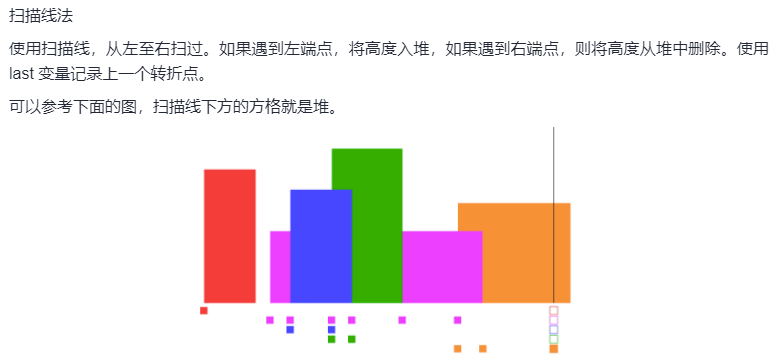
\includegraphics[width=.9\linewidth]{./pic/sweep.png}

\begin{minted}[frame=lines,fontsize=\scriptsize,linenos=false]{java}
public List<List<Integer>> getSkyline(int[][] buildings) { // 从左向右扫一遍过去
    List<List<Integer>> ans = new ArrayList<>();
    Map<Integer, List<Integer>> map = new TreeMap<>();
    for (int [] v : buildings) {
        map.computeIfAbsent(v[0], z -> new ArrayList<>()).add(-v[2]); // 插入左节点: 高度为负
        map.computeIfAbsent(v[1], z -> new ArrayList<>()).add(v[2]);  // 插入右节点:高度为正
    }
    Map<Integer, Integer> heights = new TreeMap<>((a, b) -> b-a); // 保留当前位置的所有高度 重定义排序:从大到小
    int [] last = {0, 0}; // 保留上一个位置的横坐标及高度           
    for (Integer key : map.keySet()) {
        List<Integer> ys = map.get(key);
        Collections.sort(ys);
        for (int y : ys) {
            if (y < 0) // 左端点,高度入队
                heights.put(-y, heights.getOrDefault(-y, 0) + 1);
            else {     // 右端点移除高度
                heights.put(y, heights.getOrDefault(y, 1) - 1);
                if (heights.get(y) == 0) heights.remove(y);
            }
        }
        Integer maxHeight = 0;      // 获取heights的最大值:就是第一个值
        if (!heights.isEmpty())
            maxHeight = heights.keySet().iterator().next();
        if (last[1] != maxHeight) { // 如果当前最大高度不同于上一个高度,说明其为转折点
            last[0] = key;          // 更新last,并加入结果集
            last[1] = maxHeight;
            ans.add(Arrays.asList(key, maxHeight));
        }
    }
    return ans;
}
\end{minted}

\section{715. Range Module - Hard}
\label{sec-8-4}
A Range Module is a module that tracks ranges of numbers. Design a data structure to track the ranges represented as half-open intervals and query about them.

A half-open interval [left, right) denotes all the real numbers x where left <= x < right.

Implement the RangeModule class:

RangeModule() Initializes the object of the data structure.
void addRange(int left, int right) Adds the half-open interval [left, right), tracking every real number in that interval. Adding an interval that partially overlaps with currently tracked numbers should add any numbers in the interval [left, right) that are not already tracked.
boolean queryRange(int left, int right) Returns true if every real number in the interval [left, right) is currently being tracked, and false otherwise.
void removeRange(int left, int right) Stops tracking every real number currently being tracked in the half-open interval [left, right).
\begin{minted}[frame=lines,fontsize=\scriptsize,linenos=false]{java}
    class Range {
        int left, right;
        public Range(int left, int right) {
            this.left = left;
            this.right = right;
        }
    }
    TreeSet<Range> ts;
    public RangeModule() {
        ts = new TreeSet<>((a, b)->(a.left != b.left ? a.left - b.left : a.right - b.right));
    }
    public void addRange(int left, int right) {
        int nl = left, nr = right;
        Range high = new Range(right, Integer.MAX_VALUE);
        while (true) {
            Range r = ts.lower(high);
            if (r == null || r.right < left) break;
            if (r.right > right) nr = r.right;
            if (r.left < left) nl = r.left;
            ts.remove(r);
        }
        ts.add(new Range(nl, nr));
    }
    public boolean queryRange(int left, int right) {
        Range target = ts.floor(new Range(left, Integer.MAX_VALUE));
        return target != null && target.left <= left && target.right >= right;
    }
    public void removeRange(int left, int right) {
        Range high = new Range(right, right);
        while (true) {
            Range r = ts.lower(high);
            if (r == null || r.right <= left) break;
            if (r.right > right)
                ts.add(new Range(right, r.right));
            if (r.left < left)
                ts.add(new Range(r.left, left));
            ts.remove(r);
        }
    }
\end{minted}

\section{352. Data Stream as Disjoint Intervals - Hard}
\label{sec-8-5}
Given a data stream input of non-negative integers a1, a2, \ldots{}, an, summarize the numbers seen so far as a list of disjoint intervals.

Implement the SummaryRanges class:

SummaryRanges() Initializes the object with an empty stream.
void addNum(int val) Adds the integer val to the stream.
int[][] getIntervals() Returns a summary of the integers in the stream currently as a list of disjoint intervals [starti, endi].
\begin{minted}[frame=lines,fontsize=\scriptsize,linenos=false]{java}
    class Range implements Comparable<Range> {
        int bgn, end;
        public Range(int bgn, int end) {
            this.bgn = bgn;
            this.end = end;
        }
        @Override public int compareTo(Range other) {
            return this.bgn - other.bgn;
        }
    }
    TreeSet<Range> ts; 
    public SummaryRanges() {
        ts = new TreeSet<Range>();
    }
    public void addNum(int val) {
        Range cur = new Range(val, val);
        Range bef = ts.floor(cur);
        Range aft = ts.ceiling(cur);
        if (bef != null && bef.end + 1 >= val) {
            cur.bgn = bef.bgn;
            cur.end = Math.max(val, bef.end);
            ts.remove(bef);
        }
        if (aft != null && aft.bgn == val + 1) {
            cur.end = aft.end;
            ts.remove(aft);
        }
        ts.add(cur);
    }
    public int[][] getIntervals() {
        int [][] ans = new int [ts.size()][2];
        int i = 0;
        for (Range cur : ts) {
            ans[i][0] = cur.bgn;
            ans[i][1] = cur.end;
            i++;
        }
        return ans;
    }
\end{minted}

\section{1419. Minimum Number of Frogs Croaking - Medium}
\label{sec-8-6}
Given the string croakOfFrogs, which represents a combination of the string "croak" from different frogs, that is, multiple frogs can croak at the same time, so multiple “croak” are mixed. Return the minimum number of different frogs to finish all the croak in the given string.

A valid "croak" means a frog is printing 5 letters ‘c’, ’r’, ’o’, ’a’, ’k’ sequentially. The frogs have to print all five letters to finish a croak. If the given string is not a combination of valid "croak" return -1.
\begin{minted}[frame=lines,fontsize=\scriptsize,linenos=false]{java}
public int minNumberOfFrogs(String s) { // 写得有点儿乱
    int n = s.length();
    int cc = 0, cr = 0, co = 0, ca = 0, cnt = 0, max = 0;
    for (int i = 0; i < n; i++) {
        char c = s.charAt(i);
        if (c == 'c') {
            ++cc;
            ++cnt;
            max = Math.max(max, cnt);
        } else if (c == 'r') {
            if (cc == 0) return -1;
            --cc;
            ++cr;
        } else if (c == 'o') {
            if (cr == 0) return -1;
            --cr;
            ++co;
        } else if (c == 'a') {
            if (co == 0) return -1;
            --co;
            ++ca;
        } else if (c == 'k') {
            if (ca == 0) return -1;
            --ca;
            --cnt;
        }
    }
    if (cc + cr + co + ca > 0) return -1;
    return max;
}
\end{minted}

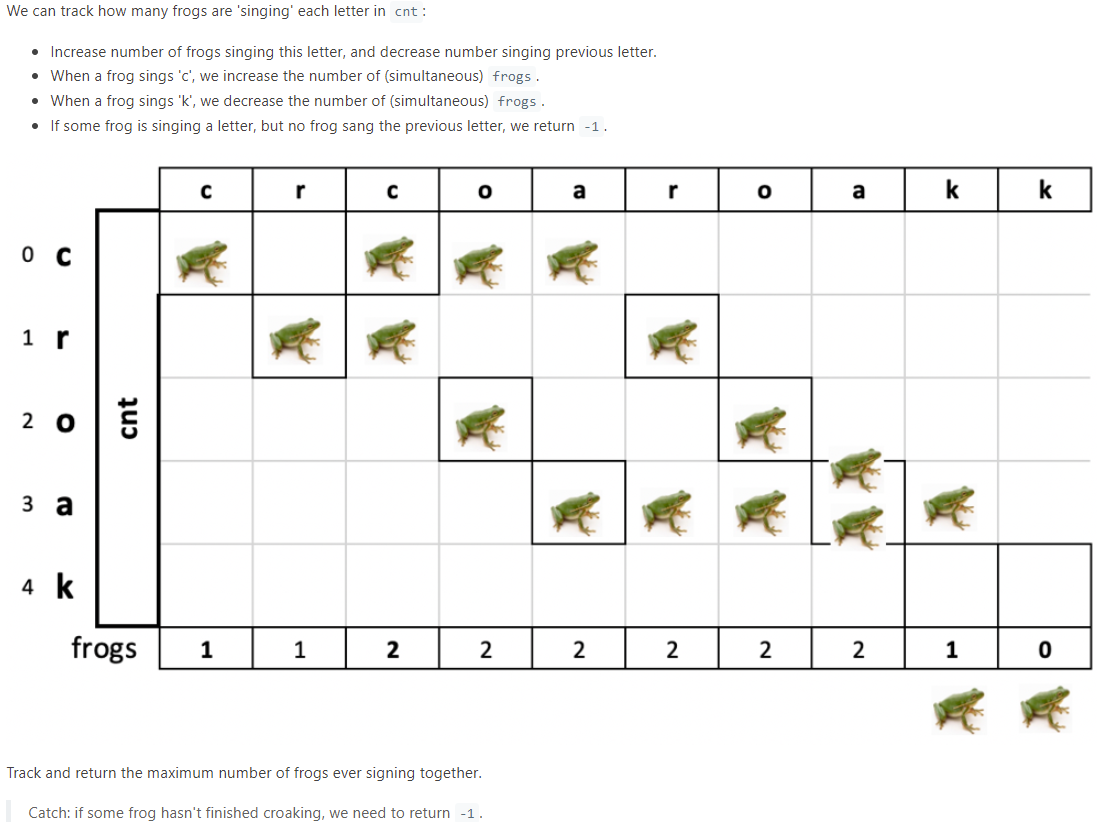
\includegraphics[width=.9\linewidth]{./pic/frogs.png}
\begin{minted}[frame=lines,fontsize=\scriptsize,linenos=false]{java}
public int minNumberOfFrogs(String s) {
    int n = s.length();
    int cnt [] = new int [5];
    int cur = 0, max = 0;
    for (int i = 0; i < n; i++) {
        char c = s.charAt(i);
        int idx = "croak".indexOf(c);
        ++cnt[idx];
        if (idx == 0)
            max = Math.max(max, ++cur);
        else if (--cnt[idx-1] < 0)
            return -1;
        else if (idx == 4)
            --cur;
    }
    return cur == 0 ? max : -1; // 如果最后所有的青蛙都叫完了的话  
}
\end{minted}
\begin{itemize}
\item 解法三:
\end{itemize}

这个跟上面的解法差不多,优化了查询位置的时间。直接对比每一步的结果。如果当前字符位的个数比上一位多,那么说明当前位没有办法被匹配成功。

\begin{minted}[frame=lines,fontsize=\scriptsize,linenos=false]{java}
public int minNumberOfFrogs(String croakOfFrogs) {
    char[] ch = croakOfFrogs.toCharArray();
    int curr = 0;
    int res = 0;
    int c = 0, r = 0, o = 0, a = 0, k = 0;
    for(int i = 0; i < ch.length; i++) {
        if(ch[i] == 'c') {
            c++;
            curr++;
        } else if(ch[i] == 'r') 
            r++;
        else if(ch[i] == 'o') 
            o++;
         else if(ch[i] == 'a') 
            a++;
         else {
            k++; 
            curr--;
        }
        res = Math.max(res, curr);
        if (c < r || r < o || o < a || a < k) // 要满足所有的条件
            return -1;
    }
    if ((c == r) && (r == o ) && ( o == a) &&  (a == k)) 
        return res;
    return -1;
}
\end{minted}


\chapter{PreSum}
\label{sec-9}
\section{1674. Minimum Moves to Make Array Complementary - Medium 差分数组}
\label{sec-9-1}
You are given an integer array nums of even length n and an integer limit. In one move, you can replace any integer from nums with another integer between 1 and limit, inclusive.

The array nums is complementary if for all indices i (0-indexed), nums[i] + nums[n - 1 - i] equals the same number. For example, the array [1,2,3,4] is complementary because for all indices i, nums[i] + nums[n - 1 - i] = 5.

Return the minimum number of moves required to make nums complementary.
\subsection{解题思路与分析 Sweep Line / Prefix Sum}
\label{sec-9-1-1}
Let a = min(nums[i], nums[n-i-1]), b = max(nums[i], nums[n-i-1])

The key to this problem is how many moves do we need to make a + b == T.
\begin{minted}[frame=lines,fontsize=\scriptsize,linenos=false]{java}
if 2 <= T < a + 1, two moves, lower both a and b.
if a +1 <= T < a + b, one move, lower b
if a + b == T, zero move
if a + b + 1 <= T < b + limit + 1, one move, increase a
if b + limit + 1 <= T <= 2*limit, two moves, increase both a and b.
\end{minted}
\begin{itemize}
\item 关键是找到五个关键点,并利用扫描线、差分数组来暴搜所有数对和,并最全局最优解
\end{itemize}

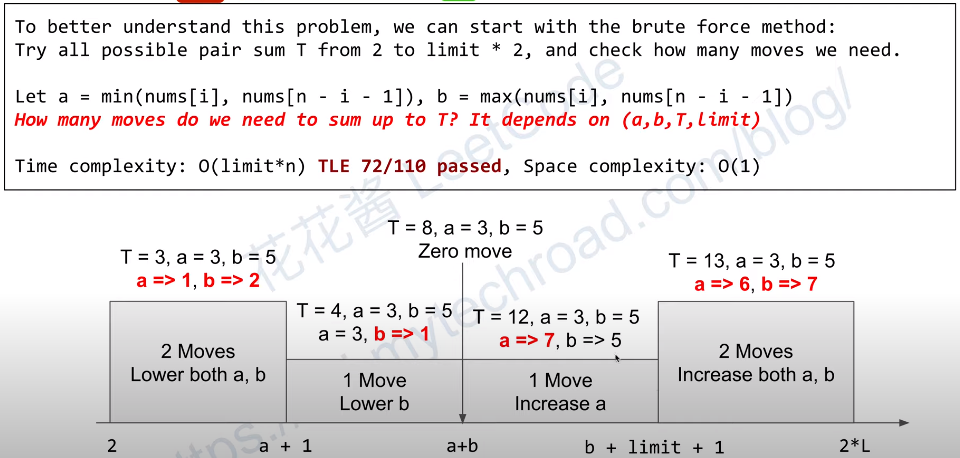
\includegraphics[width=.9\linewidth]{./pic/diffArray.png}

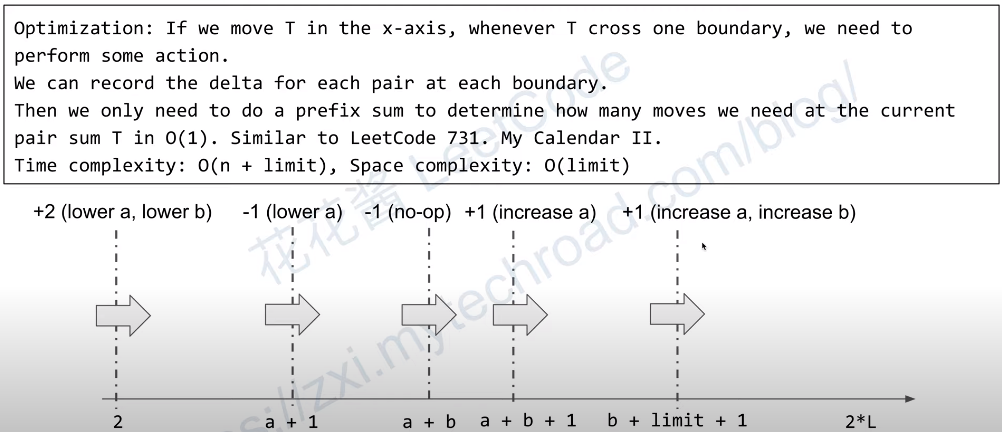
\includegraphics[width=.9\linewidth]{./pic/diffArray2.png}

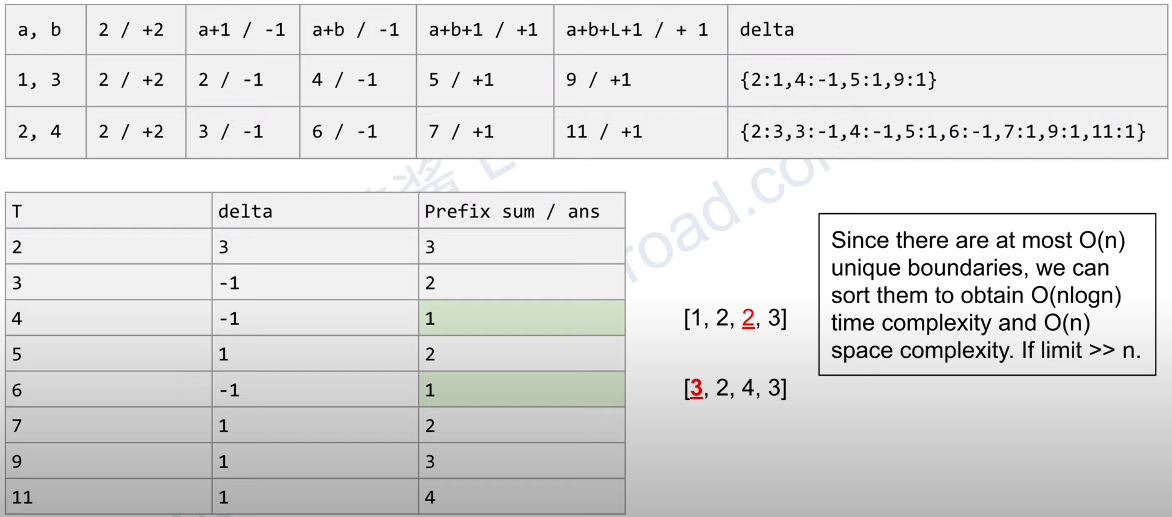
\includegraphics[width=.9\linewidth]{./pic/diffArray3.png}

\begin{minted}[frame=lines,fontsize=\scriptsize,linenos=false]{java}
public int minMoves(int[] nums, int limit) {
    int n = nums.length;
    int [] delta = new int [2 * limit + 2]; // 差分数组
    for (int i = 0; i < n/2; i++) {
        int a = Math.min(nums[i], nums[n-1-i]);
        int b = Math.max(nums[i], nums[n-1-i]); // 把各区间所需要的操作简化到五行代码中去了
        delta[2] += 2; // dec a, decreasing b [2, a] 区间的和 所需要的变换次数都是 2 次
        --delta[a+1];  // dec a               [a + 1, a+b-1] 区间中的和 所需要变的次数都是1次
        --delta[a+b];  // no operations
        ++delta[a+b+1];// inc a               [a+b+1, b+limit] 区间中的和 只需要变动 1 次;
        ++delta[b+limit+1]; // inc a, inc b
    }
    int ans = n, sum = 0;
    for (int t = 2; t < 2 * limit + 2; t++) {
        sum += delta[t]; // 差分数组的前缀和等于(共需要的操作次数)
        ans = Math.min(ans, sum);
    }
    return ans;
}
\end{minted}

\section{1074. Number of Submatrices That Sum to Target - Hard 二维数组转化为一维数组:  数组中target Sum的2D版、presum思想的2d版}
\label{sec-9-2}
Given a matrix and a target, return the number of non-empty submatrices that sum to target.

A submatrix x1, y1, x2, y2 is the set of all cells matrix[x][y] with x1 <= x <= x2 and y1 <= y <= y2.

Two submatrices (x1, y1, x2, y2) and (x1', y1', x2', y2') are different if they have some coordinate that is different: for example, if x1 != x1'.

本题也需要使用到presum思路来解题,只不过这个前缀和presum的计算对象是二维数组。对于任意一个点,presum[i][j]代表了从Matrix\footnotemark[1]{}\textsuperscript{,}\,\footnotemark[1]{}到Matrix[i][j]之间的和。

有了前缀和之后,我们可以将二维数组拆解为多个一维数组,再用一维数组的思路去解题。

拆分数组时可以以列拆分,也可以以行拆,无论如何都可以达到遍历所有子矩阵的效果。本题以列拆分为例,对于任意两列col1和col2,我们可以得到所有行的前缀和

这样,二维数组就转化为了一维数组。接下来只要遍历所有列的组合即可。
\begin{minted}[frame=lines,fontsize=\scriptsize,linenos=false]{java}
public int numSubmatrixSumTarget(int[][] matrix, int target) {
    int m = matrix.length, n = matrix[0].length, rowSum = 0;
    int [][] sum = new int [m][n]; // sums of row sum only
    for (int i = 0; i < m; i++) {
        rowSum = 0;
        for (int j = 0; j < n; j++) {
            rowSum += matrix[i][j];
            sum[i][j] = rowSum + (i == 0 ? 0 : sum[i-1][j]);
        }
    }
    int cnt = 0, cur = 0;
    for (int j = 0; j < n; j++)     // col1
        for (int k = j; k < n; k++) {// col2
            Map<Integer, Integer> map = new HashMap<>(); // 用于记录前缀和个数
            for (int i = 0; i < m; i++) {
                cur = sum[i][k] - (j == 0 ? 0 : sum[i][j-1]);
                if (cur == target) ++cnt;
                cnt += map.getOrDefault(cur - target, 0);
                map.put(cur, map.getOrDefault(cur, 0) + 1);
            }
        }
    return cnt;
}
\end{minted}
\begin{itemize}
\item 对corner case的处理相对简洁的写法
\end{itemize}
\begin{minted}[frame=lines,fontsize=\scriptsize,linenos=false]{java}
public int numSubmatrixSumTarget(int [][] matrix, int target) { 
    int res = 0, m = matrix.length, n = matrix[0].length;
    int [][] sum = new int [m+1][n+1];
    for (int i = 1; i <= m; ++i) 
        for (int j = 1; j <= n; ++j) // 对全数组纵横求和
            sum[i][j] = sum[i][j - 1] + sum[i - 1][j] - sum[i - 1][j - 1] + matrix[i - 1][j - 1];
    for (int i = 1; i <= m; ++i) 
        for (int j = 1; j <= n; ++j) 
            for (int p = 1; p <= i; ++p) 
                for (int q = 1; q <= j; ++q) {
                    int t = sum[i][j] - sum[i][q - 1] - sum[p - 1][j] + sum[p - 1][q - 1];
                    if (t == target) ++res;
                }
    return res;
}
\end{minted}
\begin{minted}[frame=lines,fontsize=\scriptsize,linenos=false]{java}
public int numSubmatrixSumTarget(int[][] matrix, int target) {
    int m = matrix.length, n = matrix[0].length;
    int [][] sum = new int [m][n+1];                // sums of row sum only
    for (int i = 0; i < m; i++) {
        for (int j = 0; j < n; j++) 
            sum[i][j+1] = sum[i][j] + matrix[i][j]; // row sums only
    }
    int cnt = 0, cur = 0;
    for (int j = 0; j < n; j++)      // col1
        for (int k = j; k < n; k++) {// col2
            cur = 0;
            Map<Integer, Integer> map = new HashMap<>(); // 用于记录前缀和个数
            map.put(0, 1);
            for (int i = 0; i < m; i++) {
                cur += sum[i][k+1] - sum[i][j];
                cnt += map.getOrDefault(cur - target, 0);
                map.put(cur, map.getOrDefault(cur, 0) + 1);
            }
        }
    return cnt;
}
\end{minted}
解题思路分析

首先对每一行,计算一个presum

然后对任意两个列, [j,k], 计算j和k之间的所有数的和, 因为对于每一行,我们已经计算了presum, 所以,

对于[j,k]之间的树,可以通过presum[i][k] - (j == 0 ? 0 : presum[i][j-1])得到某一行在[j,k]之间的值

这样, 对于任意两列[j,k]之间的数, 我们可以形成一个临时的一维数组, 表示从第0行到最后一行的数,

那么, 问题就转换成在这个一维数组里面,找一个连续子数组, 使得这些数的和是target,

那么,后面这个问题就转换成 leetcode 560

\url{http://www.noteanddata.com/leetcode-560-Subarray-Sum-Equals-K-java-solution-note.html}

所以, 这个是presum思想的2d版, 类似的题目还有leetcode 304 Range Sum Query 2D - Immutable
\begin{minted}[frame=lines,fontsize=\scriptsize,linenos=false]{java}
public int numSubmatrixSumTarget(int [][] matrix, int target) {
    int res = 0, m = matrix.length, n = matrix[0].length;
    for (int i = 0; i < m; ++i) 
        for (int j = 1; j < n; ++j) 
            matrix[i][j] += matrix[i][j - 1];
    for (int i = 0; i < n; ++i) 
        for (int j = i; j < n; ++j) {
            Map<Integer, Integer> cntMap = new HashMap<>();
            cntMap.put(0, 1);
            int cur = 0;
            for (int k = 0; k < m; ++k) {
                cur += matrix[k][j] - (i > 0 ? matrix[k][i - 1] : 0);
                res += cntMap.getOrDefault(cur-target, 0);
                cntMap.put(cur, cntMap.getOrDefault(cur, 0) + 1);
            }
        }
    return res;
}
\end{minted}
\begin{minted}[frame=lines,fontsize=\scriptsize,linenos=false]{java}
private int cntTarget(int [] arr, int target) { // 比较一下与上面解法、写法的不同!!!
    int cnt = 0, sum = 0;
    Map<Integer, Integer> cntMap = new HashMap<>();
    cntMap.put(0, 1);
    for (int i = 0; i < arr.length; i++) {
        sum += arr[i];
        cnt += cntMap.getOrDefault(sum - target, 0);
        cntMap.compute(sum, (k, v) -> { // 
                if (v == null) v = 0;
                return v+1;
            });
        return cnt;
    }
}
public int numSubmatrixSumTarget(int[][] matrix, int target) {
    int m = matrix.length, n = matrix[0].length, cur = 0;
    int [][] sum = new int [m][n]; // sums of row sum only
    for (int i = 0; i < m; i++) {
        cur = 0;
        for (int j = 0; j < n; j++) {
            cur += matrix[i][j];
            sum[i][j] = cur;
        }
    }
    int cnt = 0;
    for (int j = 0; j < n; j++) {
        for (int k = j; k < n; k++) {
            int [] tmp = new int [m];
            for (int i = 0; i < m; i++) 
                tmp[i] = sum[i][k] - (j == 0 ? 0 : sum[i][j-1]);
            int oneCnt = cntTarget(tmp, target);
            cnt += oneCnt;
        }
    }
    return cnt;
}
\end{minted}

\chapter{Greedy}
\label{sec-10}
\section{1585. Check If String Is Transformable With Substring Sort Operations - Hard}
\label{sec-10-1}
Given two strings s and t, you want to transform string s into string t using the following operation any number of times:

Choose a non-empty substring in s and sort it in-place so the characters are in ascending order.
For example, applying the operation on the underlined substring in "14234" results in "12344".

Return true if it is possible to transform string s into string t. Otherwise, return false.

A substring is a contiguous sequence of characters within a string.
\begin{minted}[frame=lines,fontsize=\scriptsize,linenos=false]{java}
public boolean isTransformable(String s, String t) { 
    ArrayDeque<Integer> [] q = new ArrayDeque[10];
    for (int i = 0; i < 10; i++) 
        q[i] = new ArrayDeque<Integer>();
    for (int i = 0; i < s.length(); i++) 
        q[s.charAt(i)-'0'].offerLast(i);
    for (char c : t.toCharArray()) {
        int d = c - '0';
        if (q[d].isEmpty()) return false;
        for (int i = 0; i < d; i++) 
            if (!q[i].isEmpty() && q[i].peekFirst() < q[d].peekFirst())
                return false;
        q[d].pollFirst();
    }
    return true;
}
\end{minted}

\section{1330. Reverse Subarray To Maximize Array Value - Hard}
\label{sec-10-2}
You are given an integer array nums. The value of this array is defined as the sum of |nums[i]-nums[i+1]| for all 0 <= i < nums.length-1.

You are allowed to select any subarray of the given array and reverse it. You can perform this operation only once.

Find maximum possible value of the final array.


\includegraphics[width=.9\linewidth]{./pic/reverseSubarray.png}

\begin{minted}[frame=lines,fontsize=\scriptsize,linenos=false]{java}
public int maxValueAfterReverse(int[] a) { 
    int n = a.length, base = 0, ans = 0, sum = 0;
    if (n == 1) return 0;
    for (int i = 0; i < n-1; i++)
        sum += abs(a[i] - a[i+1]);
    // 交换的区间左端点是数组的左边界
    for (int i = 0; i < n-1; i++) 
        ans = max(ans, sum + abs(a[i+1]-a[0]) - abs(a[i+1] - a[i]));
    // 交换的区间右端点是数组的右边界
    for (int i = n-1; i > 0; i--)
        ans = max(ans, sum + abs(a[n-1] - a[i-1]) - abs(a[i] - a[i-1]));
    // 交换区间左右端点在数组内部
    int l = 1; // 1. 找出左端点
    for (int i = 2; i < n; i++) {
        int ia = min(a[i], a[i-1]), ib = max(a[i], a[i-1]);
        if (max(a[i], a[i-1]) < max(a[l], a[l-1])) l = i;
    }
    int r = 0; // 2. 找出右端点
    for (int i = 1; i < n-1; i++) 
        if (min(a[i], a[i+1]) > min(a[r], a[r+1])) r = i;
    ans = max(ans, sum + 2 * (min(a[r], a[r+1]) - max(a[l], a[l-1])));
    return ans;
}
\end{minted}

\chapter{others}
\label{sec-11}
\section{Predict the Winner}
\label{sec-11-1}
You are given an integer array nums. Two players are playing a game with this array: player 1 and player 2.
Player 1 and player 2 take turns, with player 1 starting first. Both players start the game with a score of 0. At each turn, the player takes one of the numbers from either end of the array (i.e., nums\footnotemark[1]{} or nums[nums.length - 1]) which reduces the size of the array by 1. The player adds the chosen number to their score. The game ends when there are no more elements in the array.
Return true if Player 1 can win the game. If the scores of both players are equal, then player 1 is still the winner, and you should also return true. You may assume that both players are playing optimally.
\begin{minted}[frame=lines,fontsize=\scriptsize,linenos=false]{java}
private int helper( int [] arr, int i, int j) {
    if (i == j) return arr[i];
    else return Math.max(arr[i] - helper(arr, i+1, j), arr[j] - helper(arr, i, j-1));
}
public boolean PredictTheWinner(int[] nums) {
    int n = nums.length;
    if (n == 1) return true;
    return helper(nums, 0, n-1) >= 0;
}
\end{minted}

\section{Rectangle Area II}
\label{sec-11-2}
We are given a list of (axis-aligned) rectangles. Each rectangle[i] = [xi1, yi1, xi2, yi2] , where (xi1, yi1) are the coordinates of the bottom-left corner, and (xi2, yi2) are the coordinates of the top-right corner of the ith rectangle.
Find the total area covered by all rectangles in the plane. Since the answer may be too large, return it modulo 109 + 7.
\begin{minted}[frame=lines,fontsize=\scriptsize,linenos=false]{java}
private void addRectange(List<int[]> l, int [] arr, int idx) {
    if (idx >= l.size()) {
        l.add(arr);
        return;
    }
    int [] r = l.get(idx);
    // 新增矩形 处在 左 右 上 下 四侧完全不重叠的区域
    if (arr[2] <= r[0] || arr[0] >= r[2] || arr[1] >= r[3] || arr[3] <= r[1]) { 
        addRectange(l, arr, idx+1);
        return;
    }
    if (arr[0] < r[0]) // 新增矩形 左侧 有交叠
        addRectange(l, new int[]{arr[0], arr[1], r[0], arr[3]}, idx+1);
    if (arr[2] > r[2]) // 新增矩形 右侧 也可以有 交叠
        addRectange(l, new int[]{r[2], arr[1], arr[2], arr[3]}, idx+1);
    if (arr[1] < r[1]) // 新增矩形 下侧 也可以有 交叠: 注意左侧、右侧前面已经加进去了,现在只加中间部分,不要重复计算
        addRectange(l, new int[]{Math.max(arr[0], r[0]), arr[1], Math.min(arr[2], r[2]), r[1]}, idx+1);
    if (arr[3] > r[3]) // 新增矩形 上侧 也可以有 交叠: 注意左侧、右侧、下侧 前面已经加进去了,现在只加中间部分,不要重复计算
        addRectange(l, new int[]{Math.max(arr[0], r[0]), r[3], Math.min(arr[2], r[2]), arr[3]}, idx+1);
}
public int rectangleArea(int[][] rectangles) {
    int mod = (int)Math.pow(10, 9)+7;
    long res = 0;
    List<int[]> rlist = new ArrayList<>();
    for (int [] val : rectangles) 
        addRectange(rlist, val, 0);
    for (int [] arr : rlist) 
        res = (res + ((long)(arr[2]-arr[0])*(long)(arr[3]-arr[1]))) % mod;
    return (int)res % mod;
}
\end{minted}

\section{Construct Binary Tree from Preorder and Postorder Traversal}
\label{sec-11-3}
Given two integer arrays, preorder and postorder where preorder is the preorder traversal of a binary tree of distinct values and postorder is the postorder traversal of the same tree, reconstruct and return the binary tree.
If there exist multiple answers, you can return any of them.
\begin{minted}[frame=lines,fontsize=\scriptsize,linenos=false]{java}
public TreeNode constructFromPrePost(int[] preorder, int[] postorder) {
    int n = preorder.length;
    TreeNode r = new TreeNode(preorder[0]);
    if (n == 1) return r;
    Stack<TreeNode> s = new Stack<>();
    s.push(r);
    int idx = 0;
    for (int i = 1; i < n; i++) {
        TreeNode cur = new TreeNode(preorder[i]);
        if (s.peek().left == null) s.peek().left = cur;
        else s.peek().right = cur;
        s.push(cur);
        while (idx < n && postorder[idx] == s.peek().val) {
            s.pop();
            ++idx;
        }
    }
    return r;
}
\end{minted}

\section{Path Sum III}
\label{sec-11-4}
Given the root of a binary tree and an integer targetSum, return the number of paths where the sum of the values along the path equals targetSum.
The path does not need to start or end at the root or a leaf, but it must go downwards (i.e., traveling only from parent nodes to child nodes).
\begin{minted}[frame=lines,fontsize=\scriptsize,linenos=false]{java}
private int solve(TreeNode r, int t, int value) {
    if (r == null) return 0;
    if (value + r.val == t)
        return 1 + solve(r.left, 0, 0) + solve(r.right, 0, 0);
    return solve(r.left, t, value + r.val) + solve(r.right, t, value + r.val);
}
public int pathSum(TreeNode root, int targetSum) {
    if (root == null) return 0;
    return solve(root, targetSum, 0) + pathSum(root.left, targetSum) + pathSum(root.right, targetSum);
}
\end{minted}

\section{Critical Connections in a Network}
\label{sec-11-5}
\begin{itemize}
\item There are n servers numbered from 0 to n - 1 connected by undirected server-to-server connections forming a network where connections[i] = [ai, bi] represents a connection between servers ai and bi. Any server can reach other servers directly or indirectly through the network.
\item A critical connection is a connection that, if removed, will make some servers unable to reach some other server.
\item Return all critical connections in the network in any order.
\end{itemize}
\begin{minted}[frame=lines,fontsize=\scriptsize,linenos=false]{java}
static class Eg {
    int u, v, next;
    // int w;
    boolean cut;
    // int num;
}
public Eg[] egs;
public int cnt;
public int [] fir; // 边的出发点
int [] low;
int [] dfn;
int recdfn;
void tarjanAddEg(int u, int v, int w) {
    egs[cnt] = new Eg();
    egs[cnt].u = u;
    egs[cnt].v = v;
    // egs[cnt].w = w;
    egs[cnt].cut = false;
    // egs[cnt].num = 0;
    egs[cnt].next = fir[u]; // ?
    fir[u] = cnt++;         // ?
}
private void initTarjan(int nodeSize, int edgeSize) {
    cnt = 0;
    egs = new Eg [edgeSize];
    low = new int [nodeSize];
    dfn = new int [nodeSize];
    fir = new int [edgeSize];
    Arrays.fill(fir, -1);
}
private void tarjan(int u, int fa) { // fa: father
    low[u] = ++recdfn;
    dfn[u] = recdfn;
    int have = 0;
    for (int i = fir[u]; i != -1; i = egs[i].next) {
        int v = egs[i].v;
        if (have == 0 && v == fa) { // 走过你来时的路
            have++;
            continue;
        }
        if (dfn[v] == 0) { // dfs过程中还未经过该点
            tarjan(v, u);
            low[u] = Math.min(low[u], low[v]);
            if (dfn[u] < low[v]) { // 连通世外桃源与外界的路
                // 当 dfn[x] < low[y] 的时候:
                // --- 我们发现从yy节点出发,在不经过(x,y)(x,y)的前提下,不管走哪一条边,我们都无法抵达xx节点,或者比xx节点更早出现的节点
                // --- 此时我们发现yy所在的子树似乎形成了一个封闭圈,那么(x,y)(x,y)自然也就是桥了.
                egs[i].cut = true;
                egs[i^1].cut = true; // ???
            }
        } else {
            low[u] = Math.min(low[u], dfn[v]); // 取已访问的节点的dfs序的最小值
        }
    }
}
private boolean findEdgeCut(int l, int r) {
    Arrays.fill(low, 0);
    Arrays.fill(dfn, 0);
    recdfn = 0;
    tarjan(l, l);
    for (int i = l; i <= r; i++) {
        if (dfn[i] == 0) return false;
    }
    return true;
}
public List<List<Integer>> criticalConnections(int n, List<List<Integer>> connections) {
    initTarjan(n, connections.size()*2);
    for (List<Integer> eg : connections) {
        tarjanAddEg(eg.get(0), eg.get(1), 1);
        tarjanAddEg(eg.get(1), eg.get(0), 1);
    }
    // boolean ans = findEdgeCut(0, n-1);
    Arrays.fill(low, 0);
    Arrays.fill(dfn, 0);
    recdfn = 0;
    tarjan(0, 0);
    List<List<Integer>> res = new ArrayList<>();
    int l = connections.size();
    for (int i = 0; i < l * 2; i += 2) { // i += 2 skipped egs[i^1] ?
        Eg eg = egs[i];
        if (eg != null && eg.cut) {
            List<Integer> t = new ArrayList<>();
            t.add(eg.u);
            t.add(eg.v);
            res.add(t);
        }
    }
    return res;
}
\end{minted}
% Emacs 27.1 (Org mode 8.2.7c)
\end{document}